\documentclass[10pt, twoside]{article}
\usepackage{setspace,enumerate}
\usepackage{helvet, textcomp}
\usepackage{graphicx}
\usepackage[labelfont=bf]{caption}
\usepackage{lineno, hyperref}
\usepackage[utf8]{inputenc}
\usepackage[table,xcdraw]{xcolor}
\usepackage{multirow}
\usepackage{float, subfig}
\usepackage{manyfoot, booktabs, listings}
\usepackage{algorithm,algorithmicx,algpseudocode}
\usepackage{amsmath,amssymb,amsfonts,amsthm,mathrsfs}%
\usepackage{stmaryrd, wrapfig}
\usepackage{geometry}

\geometry{letterpaper, portrait, margin=1in}
\hypersetup{colorlinks=true, linkcolor=blue, filecolor=blue, urlcolor=blue, citecolor=blue}

\usepackage[title]{appendix}
\usepackage[sort&compress,numbers]{natbib}
\bibliographystyle{unsrtnat}

\raggedbottom
\linenumbers

\begin{document}

\doublespacing

\begin{center}
    {\huge Stochastic pix2vid: A new spatiotemporal deep learning method for image-to-video synthesis in geologic CO$_2$ storage prediction}
    \vspace{5mm}
    
    \textbf{Misael M. Morales$^{1*}$}, 
    \textbf{Carlos Torres-Verd\'in$^{1,2}$}, and
    \textbf{Michael J. Pyrcz$^{1,2}$}
\end{center}

\begin{flushleft}
    1. Hildebrand Department of Petroleum and Geosystems Engineering, The University of Texas at Austin
    2. Jackson School of Geosciences, The University of Texas at Austin
    
    *Corresponding author; email: \url{misaelmorales@utexas.edu}
\end{flushleft}

%%==================================%%
%%              ABSTRACT            %%
%%==================================%%
\section*{\textbf{Abstract}}
Numerical simulation of multiphase flow in porous media is an important step in understanding the dynamic behavior of geologic CO$_2$ storage (GCS). Scaling up GCS requires fast and accurate high-resolution modeling of the storage reservoir pressure and saturation plume migration; however, such modeling is challenging due to the high computational costs of traditional physics-based simulations. Deep learning models trained with numerical simulation data can provide a fast and reliable alternative to expensive physics-based numerical simulations. We propose a Stochastic pix2vid neural network architecture for solving multiphase fluid flow problems with superior speed, accuracy, and efficiency. The Stochastic pix2vid model is designed based on the principles of computer vision and video synthesis and is able to generate dynamic spatiotemporal predictions of fluid flow from static reservoir models, closely mimicking the performance of traditional numerical simulation. We apply the Stochastic pix2vid model to a highly-complex CO$_2$-water multiphase problem with a wide range of reservoir models in terms of porosity and permeability heterogeneity, facies distribution, and injection configurations. The Stochastic pix2vid method is first-of-its-kind in static-to-dynamic prediction of reservoir behavior, where a single static input is mapped to its dynamic response. The Stochastic pix2vid method provides superior performance in highly heterogeneous geologic formations and complex estimation such as CO$_2$ saturation and pressure buildup plume determination. The trained model can serve as a general-purpose, static-to-dynamic (image-to-video) alternative to traditional numerical reservoir simulation of 2D CO$_2$ injection problems with up to 6,500$\times$ speedup compared to traditional numerical simulation.

\textbf{Keywords:} Image-to-video synthesis, Spatiotemporal prediction, Convolutional neural network, Recurrent neural network, Proxy model

%%==================================%%
%%           INTRODUCTION           %%
%%==================================%%
\section*{\textbf{1 Introduction}}
Geologic CO$_2$ sequestration (GCS) has emerged as a potential technology solution to reduce anthropogenic greenhouse gas emissions to the atmosphere \cite{Michael2010, Goodman2013329, Levine201681}, and has become increasingly popular worldwide due to the need to meet international climate protection agreements \cite{metz2005ipcc, Energy20202010EuropeanCommission, Unitednations2015AgreementP}. Modeling injected CO$_2$ movement in the subsurface over and beyond the life of the project is a critical component to support optimum GCS project decision making for safe and secure CO$_2$ sequestration. A schematic of typical GCS operations is shown in Figure \ref{co2types}, including storage in depleted oil and gas reservoir and deep saline formations, and CO$_2$ enhanced oil and coalbed methane recovery \cite{Bachu2015188, Tapia2016337, Castelletto2013570}. However, there are several technical challenges associated with the subsurface modeling to support GCS operations. To accurately forecast and monitor subsurface multiphase flow, physics-based high-fidelity numerical simulations are required. These numerical simulations are computationally intensive and time-consuming since they require iterative solutions of nonlinear systems of equations applied over large volumes of the subsurface at sufficient resolution to represent heterogeneity \cite{rustamzade2023, Rashid201321, Luo2011759, 2021AGUFM.H25O1207S}. Also, due to the large degree of uncertainty in subsurface data, and the spatial distribution of the properties of heterogeneous porous media between the sparsely sampled data, GCS operations require a robust probabilistic-based uncertainty assessment for improved engineering decision-making \cite{Chen2018, Sun2019, Chen2020}. In order to capture the fine-scale multiphase flow behavior given an uncertain spatial distribution of subsurface properties, a large number of numerical simulations are required, leading to very high computational costs and delayed feedback unable to support timely decision making \cite{Li2015389, Jiang2023}. 

\begin{figure}
    \centering
    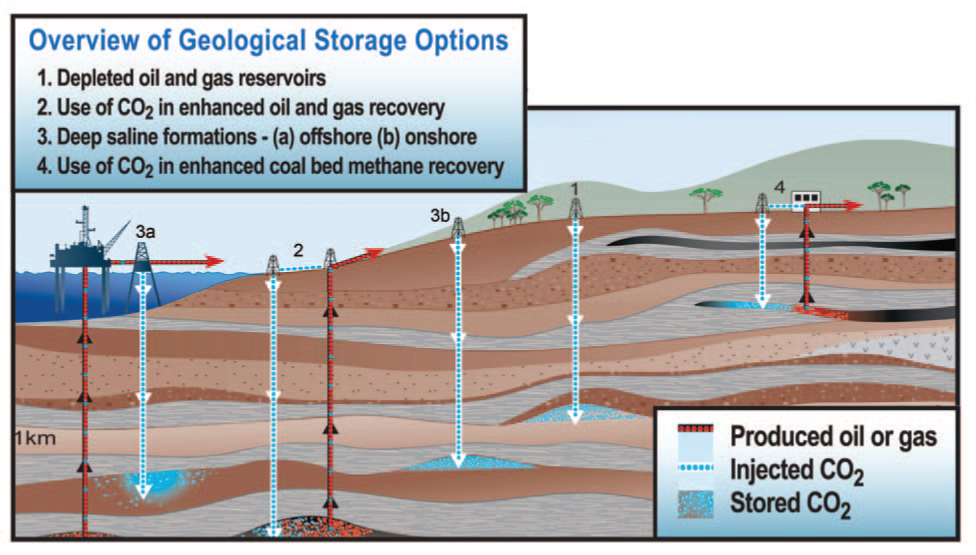
\includegraphics[width=15cm]{figures/co2types.png}
    \caption{Types of geologic CO$_2$ storage operations and the geologic formations that can be used for sequestration. \textit{Modified from the Carbon Dioxide Cooperative Research Center (CO2CRC), http://www.co2crc.com.au/about/co2crc}}
    \label{co2types}
\end{figure}

To overcome this, machine learning techniques have emerged as candidate proxy models due to their ability to perform dimensionality reduction for efficient problem parameterization and model complicated systems to calculate fast predictions of subsurface flow and transport behavior for real-time feedback on the impact of geological and engineering controls on CO$_2$ behavior in the subsurface over time \cite{10.30632/SPWLA-2023-0084, Wu2021, Misra2022}. Dimensionality reduction techniques are supervised or unsupervised machine learning methods that compress (or encode) the data, $X$, into a lower-dimensional latent feature representation, $z$, and decompress (or decode) the latent representation either: (1) back to the original data space, $\hat{X}$ (unsupervised, AutoEncoder), or (2) to a new response feature space, $y$ (supervised, Encoder-Decoder) \cite{mabadeje2023rigid, Liu2022, Canchumuni201987}, as shown in Figure \ref{latentAE}. The recent advancements in deep learning algorithms and in computing architecture and power, enable GPU-enabled neural network models that have accelerated the fields of forward and inverse modeling \cite{Zhang20111631, Yan2022}. Classical statistical modeling methods are often hindered by the size of the models and their conditioning to big data, i.e., that is data with volume, velocity, variety, value, and veracity \cite{tariq2021systematic, MIRZA202227}, and fail to generalize beyond fit-for-purpose frameworks \cite{chiles2012geostatistics, pyrcz2014geostatistical}. By analyzing big data sets, machine learning techniques can uncover complex patterns and relationships in lower-dimensional, latent feature representations that may not be discernible through traditional statistical and geostatistical methods \cite{Brunton2016SparseNLDynamics, FriesChoi2022LaSDI, HeChoi2023gLaSDI}. When combined with a latent space modeling framework, machine learning approaches efficiently and accurately exploit hidden patterns and features in the data, remove redundancies or noise, and decrease the mathematical and computational complexity of the problem significantly \cite{Liu2020M15, Razak2022}. 

\begin{figure}
    \centering
    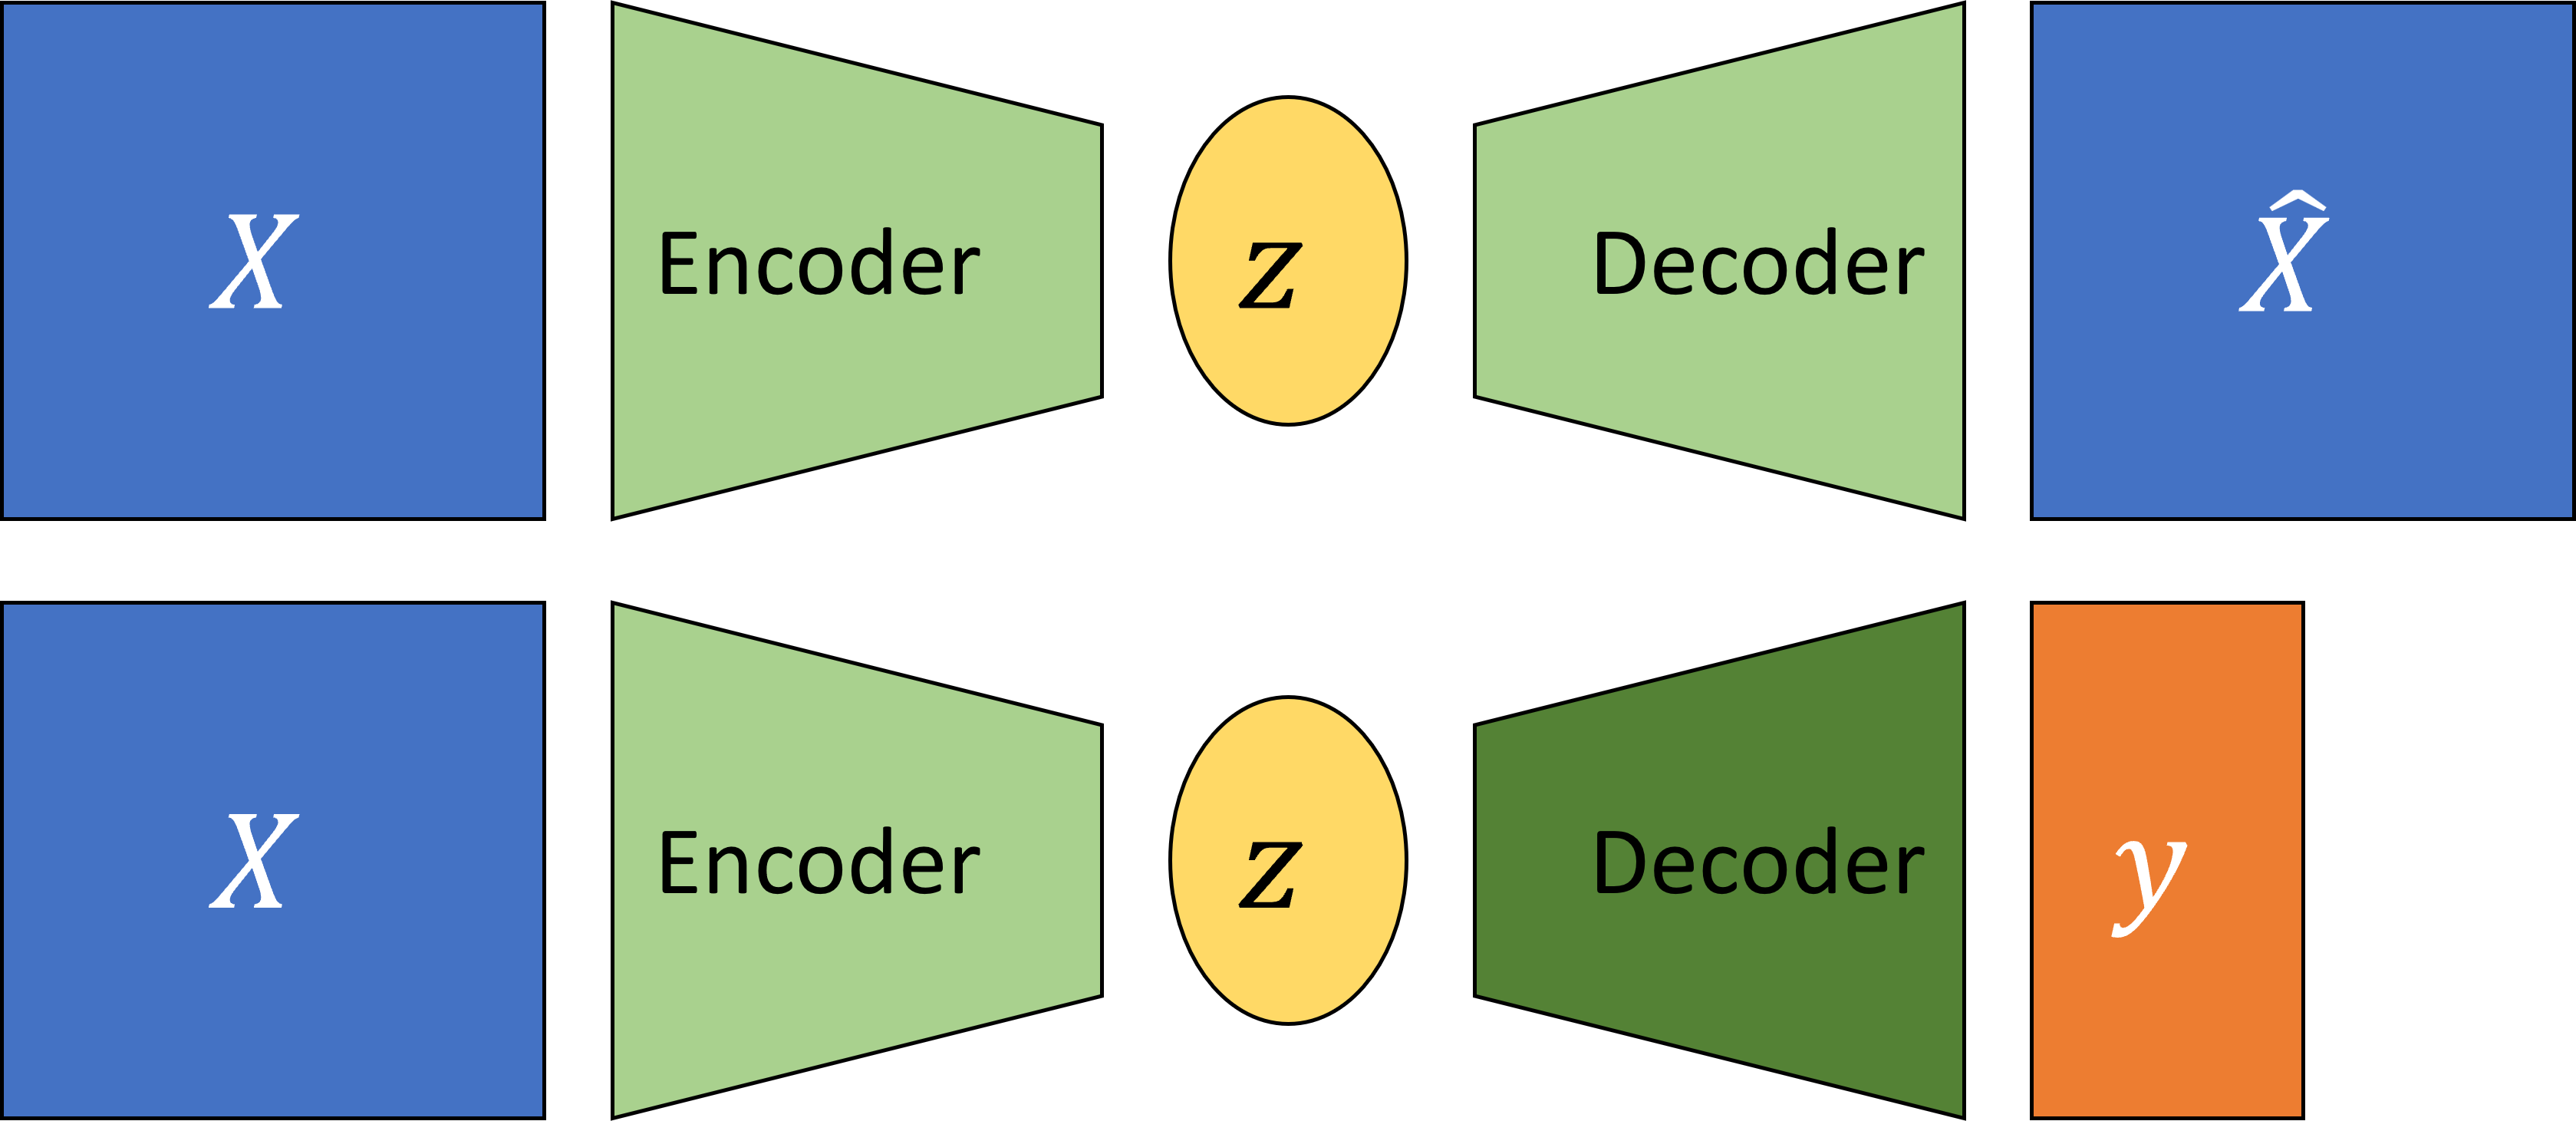
\includegraphics[width=10cm]{figures/latentAE.png}
    \caption{Dimensionality reduction model structures. Unsupervised AutoEncoder structure (top), and supervised Encoder-Decoder structure (bottom).}
    \label{latentAE}
\end{figure}

Supervised machine learning approaches applied to the subsurface are divided into two main categories, namely purely data-driven models or physics-informed models. Data-driven proxy models are neural network architectures trained with labeled data that produce a mapping from input predictor feature to output response features \cite{Oladyshkin2013671, Bao2019}. On the other hand, the training process to match training data for PINNs is regularized with the minimization of the (physical) loss from the residual of the governing partial differential equations (PDEs) along with the losses associated with the initial and boundary conditions \cite{karniadakis2021physics, yang2018physicsinformed}. However, other variants of PINNs such as physics-guided or physics-constrained neural networks where the PDE loss is not embedded in the training step, instead the models have specific architectures or parameters to mimic the physics in the system, have proven useful for subsurface energy resource engineering applications \cite{Wang2021, Coutinho2021, Zhu_2019}. One disadvantage of machine learning techniques is that they require significant
amounts of training data, but once trained these prediction models suffer from lack of generalization, i.e., inability to provide accurate predictions away from the training data beyond which they have been specifically trained \cite{Yegnanarayana2009ArtificialNetworks, heaton2018ian}. For both data-driven and physics-informed approaches, typically, spatial relationships are modeled through convolutional neural networks (CNNs) \cite{liu20213d, Yang2022} and the temporal relationships through recurrent neural networks (RNNs) \cite{jiang2021data, Ning2022}, but recent advancements in transformer-based architectures improve performance compared to the CNN and RNN methods for spatial and temporal latent feature representations \cite{liu2021swin, 10.1190/geo2022-0150.1, maldonado4403939multi}.

A number of machine learning-based proxy models have been developed to estimate the reservoir behavior in subsurface energy resource applications. Most techniques rely on the concept of image translation, or pix2pix, where a target image(s) is predicted from an input image(s) \cite{Pan2021, Sebacher2022, Bao2022, Ronneberger2015}, as shown in Figure \ref{pix2N}. \citet{Maldonado2021Unet} develop a convolutional U-Net model to predict pressure and saturation states given an uncertain geologic realization. This work is an example of image-to-image static forecasting, where the time state is given as an input, and the proxy model will predict a single response state of pressure and saturation at the given time. \citet{WEN2022104180} develop a Fourier Neural Operator (FNO) architecture to predict image-to-image response states of pressure and saturation from an uncertain geologic realization and is further extended for multi-scale and nested domains \cite{Wen2023Operators}. These methods are based on a pix2pix, or image-to-image prediction, where a specific timestep is used as an input feature to predict the relationship between the geologic model and the reservoir response at that specific timestep. This implies that pix2pix or image-to-image methods are formulated as an even-determined or sometimes over-determined estimation problem, where the number of input features is equal to or greater than the number of output features. Moreover, numerous other proxy models have been developed for subsurface applications using more complex architectures such as generative adversarial networks (GANs) \cite{jo2021machine} and transformers \cite{zhang2023evaluating, zhang2023efficient}. Despite showing consistent results and significant speedups compared to traditional numerical simulation, pix2pix models do not capture the spatiotemporal relationships and dynamic response of the subsurface system.

\begin{figure}
    \centering
    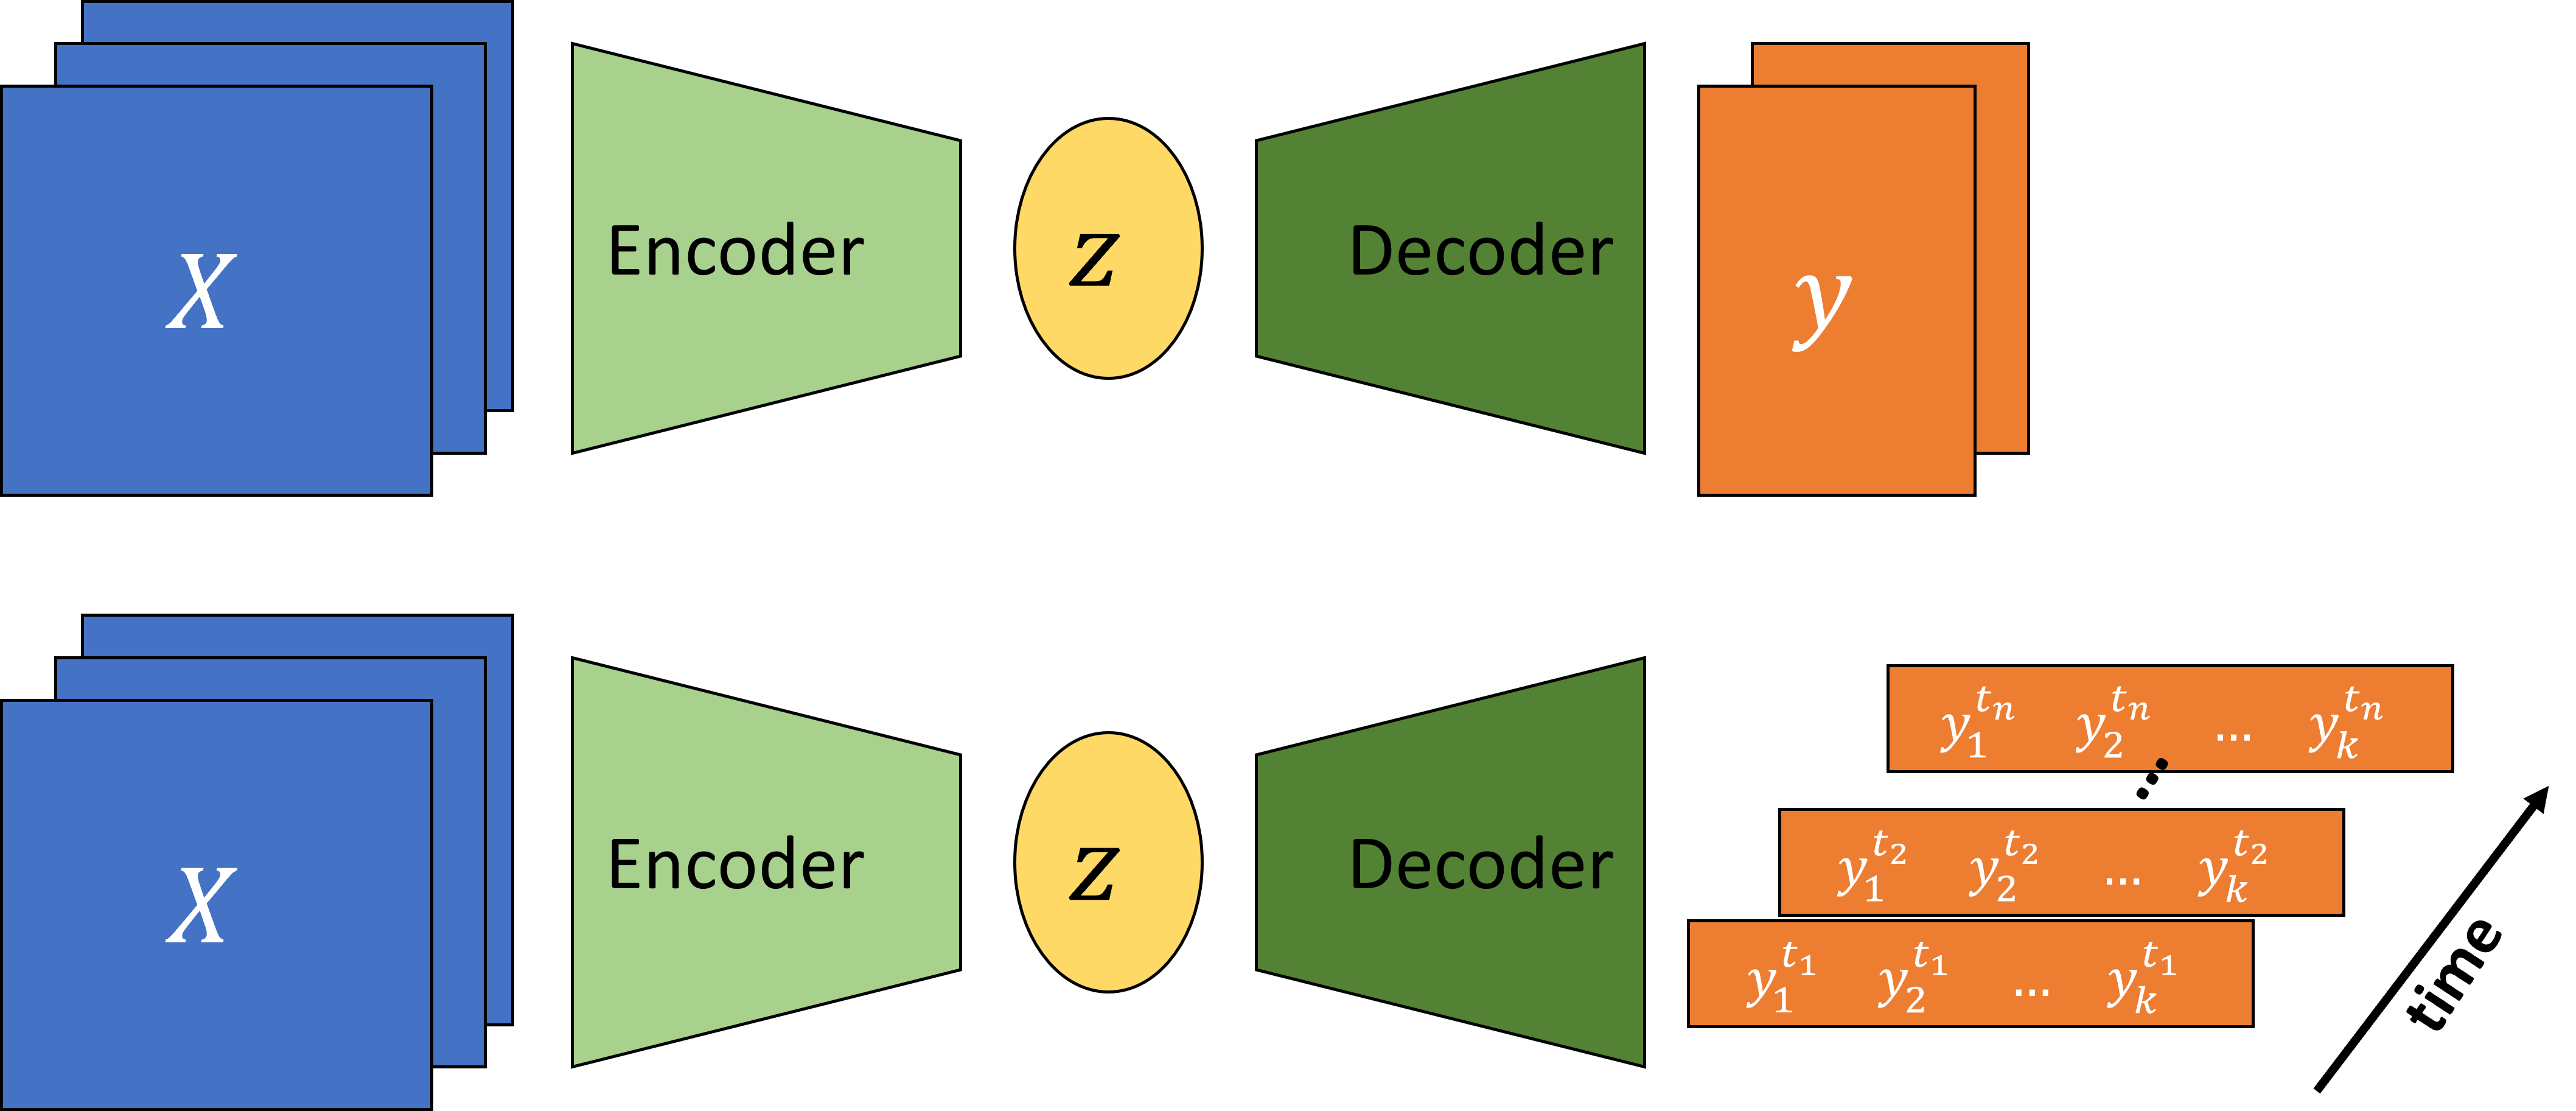
\includegraphics[width=13.5cm]{figures/pix2N.png}
    \caption{Image-to-image (pix2pix) (top) and image-to-timeseries (bottom) Encoder-Decoder structures.}
    \label{pix2N}
\end{figure}

Moving beyond image-to-image predictions, \citet{Kim2023} develop a convolutional-recurrent proxy for pix2time, or image-to-timeseries, forecasting and discuss its advantages for closed-loop reservoir management under geologic uncertainty. This method moves beyond the image-to-image forecasting and exploits a spatiotemporal latent space in an encoder-recurrent neural network architecture to obtain hydrocarbon production forecasts. The image-to-series formulation can still be an even- or over-determined estimation problem, where we have equal or more inputs than outputs, as shown in Figure \ref{pix2N}. Furthermore, \citet{Tang2020, Tang2021} and \citet{Jiang2023} develop a recurrent residual U-net (R-U-net) proxy for the prediction of dynamic pressure- and saturation-over-time from uncertain geologic realizations using an encoder-recurrent-decoder architecture. These methods aim to obtain dynamic response states over time from a single static image. This type of proxy model is formulated to resolve the more complex under-determined estimation problem (compared to even- or over-determined), where the number of input features is a fraction of the number of output features. However, the recurrent R-U-net proxy is limited by the fact that only the latent space receives spatiotemporal processing, while the model reconstruction is done via time-distributed deconvolutions, treating time as an additional “spatial” dimension, and not fully exploiting the spatiotemporal relations in the data and latent space as an image-to-video forecasting formulation.

The problem of image-to-video forecasting, also known as video synthesis, has been approached previously by researchers in the field of computer vision \cite{vondrick2016generating, mathieu2016deep, villegas2018decomposing, tulyakov2017mocogan, NIPS2015_07563a3f}. \citet{iliadis2017deep} are one of the first to develop a deep learning-based framework for video compressive sensing to reconstruct a video sequence from a single image using a deep fully-connected neural network, or artificial neural network (ANN). Despite excellent accuracy in the video predictions, this method is still limited by time-distributed fully-connected layers in the encoder and decoder portions of the network, thus not exploiting the spatiotemporal relationships in the data. \citet{xu2018csvideonet} develop a three-part encoder-recurrent-decoder network for video reconstruction from the estimated motion fields of the encoded frames. The implementation is similar to that of \citet{Jiang2023} and \citet{Tang2020, Tang2021} in that it applies a recurrent update in the latent space but relies on time-distributed deconvolutions for the video frames reconstruction to exploit spatiotemporal relationships in the data. \citet{dorkenwald2021stochastic} develop a conditional invertible neural network (cINN) as a bijective mapping between image and video domains using a dynamic latent representation. The cINN architecture allows for video-to-image and image-to-video predictions, demonstrating possible the generation of video frames from a static input image. Finally, \citet{holynski2020animating} implemented the idea of Eulerian motion fields to define the moving portions of the image to accurately reconstruct a series of video frames from a static image using a spatiotemporal latent space parameterization. These advancements in the field of computer vision and video compressed sensing are the foundation for our image-to-video proxy model.

We propose a novel image-to-video spatiotemporal proxy model, Stochastic pix2vid, for the prediction of dynamic reservoir behavior over time from a subsurface uncertainty model suite of static geologic realizations. Our model exploits the spatial and temporal structures in latent space to dynamically reconstruct the time-dependent pressure and multiphase saturation states from a static geologic realization. The model then reconstructs the dynamic pressure and saturation distributions using a spatiotemporal decoder network with convolutional long short-term memory (ConvLSTM) layers, which are concatenated with the residuals of the spatial latent parameterizations from the encoder network. Thus, it is not an encoder-recurrent-decoder architecture, but instead a fully spatiotemporal convolutional-recurrent image-to-video synthesis model. Our stochastic pix2vid model has significant advantages compared to image-to-image and encoder-recurrent-decoder models in terms of computational efficiency and prediction accuracy and can be used as a replacement for physics-based numerical reservoir simulations, or high-fidelity simulations (HFS), in GCS projects as an image-to-video mapping operator. 

In the methodology section, we describe the governing equations of multiphase flow in GCS, and the proposed spatiotemporal proxy model architecture. In the results and discussion sections, we describe the geologic modeling and numerical reservoir simulation steps required to generate the training data, and evaluate the training and performance of the proposed proxy model and compare its efficiency and accuracy to high-fidelity numerical simulations using a 2D synthetic case for large-scale GCS operations. 

%%==================================%%
%%            METHODOLOGY           %%
%%==================================%%
\section*{\textbf{2 Methodology}}
This section describes the governing equations, and the architecture and training strategy of the Stochastic pix2vid model.

%%========= subsection 2.1 =========%%
\textbf{2.1 Governing equations} 
For the CO$_2$-water multiphase flow problem, the general form of the mass accumulation for component $\kappa$ = CO$_2$ or water is given by \cite{pruess1999tough2}:

\begin{equation} \label{eq1}
    \frac{\partial M^k}{\partial t} = -\nabla \bullet F^\kappa + q^\kappa .
\end{equation}

For each component $\kappa$, the mass accumulation term $M^\kappa$ is summed over all phases $p$,

\begin{equation} \label{eq2}
    M^k = \phi \sum_p S_p \rho_p X_p^\kappa
\end{equation}

where $\phi$ is the porosity, $S_p$ is the saturation of phase $p$, $\rho_p$ is the density of phase $p$, and $X_p^\kappa$ is the mass fraction of component $\kappa$ present in phase $p$. For each component $\kappa$, there is also the advective mass flux $F^\kappa \rvert_{adv}$ obtained by summing over all phases $p$, 

\begin{equation} \label{eq3}
    F^\kappa \rvert_{adv} = \sum_p X_p^\kappa F_p
\end{equation}

where each individual phase flux $F_p$ is given by Darcy's equation:

\begin{equation} \label{eq4}
    F_p = \rho_p u_p = -k \frac{k_{r,p} \rho_p}{\mu_p} (\nabla P_p - \rho_p g)
\end{equation}

where $u_p$ is the Darcy velocity of phase $p$, $k$ is the absolute permeability, $k_{r,p}$ is the relative permeability of phase $p$, $\mu_p$ is the viscosity of phase $p$, and $g$ is the gravitational acceleration constant. The relative permeability curves for the CO$_2$-water system are shown in Figure \ref{relperms}. The fluid pressure of phase $p$,

\begin{equation} \label{eq5}
    P_p = P + P_c
\end{equation}

\begin{figure}
    \centering
    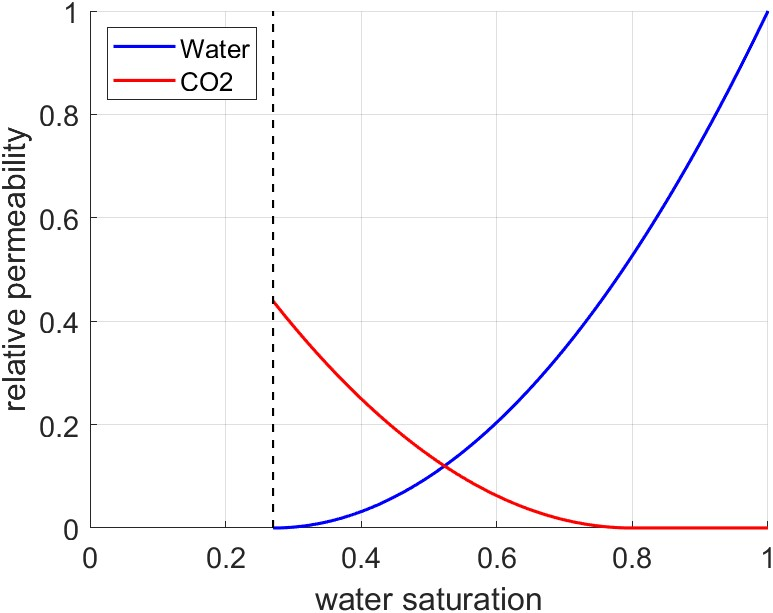
\includegraphics[width=8.5cm]{figures/relperms.jpg}
    \caption{Relative permeability curves for the CO$_2$-water system. The residual saturations are 0.27 and 0.2 for water and CO$_2$, respectively.}
    \label{relperms}
\end{figure}

is given by the sum of the reference phase pressure $P$ and the capillary pressure $P_c$. The numerical simulation does not include molecular diffusion or hydrodynamic dispersion effects for practical purposes.

%%========= subsection 2.2 =========%%
\textbf{2.2 Proxy Model Architecture} 

Our proposed Stochastic pix2vid image-to-video data-driven method, is mapping operator from the static realizations of geologic distributions of porosity, permeability and facies as well as the injector well(s) distribution, to the dynamic responses of pressure and saturation distributions over time. 

Let $m$ represent a geologic model realization of porosity, permeability, facies, and injector well(s) distributions, such that $m = \{\phi,k,facies,w\}$. The dynamic responses of pressure and saturation over time are given by $d=f(m)$, such that $d=\{P(t), S(t)\}$ and $f$ is the physics-based numerical reservoir simulation. Our aim is to replace $f$ with a more efficient data-driven proxy by training the Stochastic pix2vid model, which is trained as a single model to predict both pressure and saturation distributions over time as a multi-channel output from the multi-channel input features, $m$. For this purpose, we exploit the latent structures in space and time of the static inputs and dynamic outputs through a spatiotemporal encoder-decoder architecture. 

The encoder portion of the network is comprised of sequential convolutional layers to compress the spatial features of the subsurface realizations into a latent parameterization $z_m$, given by $z_m=Enc(m)$. In their compressed representation, these features represent the salient characteristics of the geologic distributions. The decoder portion of the network is designed as a series of recursive residual convolutional-recurrent layers, such that the latent space $z_m$ is recursively decoded into the dynamic distributions of pressure and saturation over time. The previous timestep latent representations, $z_d^t$, are used in the subsequent timesteps of the decoder, such that the subsequent timesteps will predict the current and previous timestep(s) jointly and iteratively, providing a reduction of systematic error in time as subsequent frames of the dynamic output video are predicted. The full architecture is represented as:

\begin{equation} \label{eq6}
    \hat{d} = Dec^t ( [ Enc(m) ; z_d^t ] )
\end{equation}

The encoder, $Enc(\cdot)$, compresses the geologic realizations, $m$, into a latent representation $z_m$ through the use of depthwise separable convolutions \cite{chollet2017xception}. This type of convolution learns the parameters for each channel in the image separately, avoiding mixing of variables or loss of resolution, as shown in Figure \ref{sepconv}. This is especially important when dealing with discrete, non-smooth porosity and permeability spatial distributions due to discrete facies and binary well(s) location distributions. Each separable convolution layer is regularized with an $l_1$-norm weight of $1\times10^{-6}$. Moreover, we use a Squeeze-and-Excite layer to improve channel interdependence, and to avoid mixing and loss of resolution \cite{hu2018squeeze}. Each Squeeze-and-Excite layer will provide the optimal network weights for each channel independent of the other channels by passing the feature maps through a global pooling layer (squeeze) and a dense layer with nonlinear activation (excite), to add content aware mechanism for re-weighting each channel adaptively, as shown in Figure \ref{squeeze-excite}. Furthermore, by applying instance normalization, as opposed to the more common batch normalization, we achieve channel-independent normalization of the convolved features \cite{ulyanov2016instance}. Instance normalization is a special case of group normalization, where the numbers of channels per group is exactly 1, such that each channels gets its own normalization scheme, as shown in Figure \ref{instance-norm}. Parametric rectified linear units (PReLU) is used as the activation function, where at each minibatch iteration, the network learns the optimal leaky slope for activation in each layer, as shown in Figure \ref{prelu}. Finally, pooling and spatial dropout are applied to reduce in half the input dimension of each layer and to provide a means of spatial regularization, respectively. Through 3 convolutional encoding layers with filter size $3\times3$, we obtain the latent parameterizations $z_m^1$, $z_m^2$, and $z_m^3$. Table \ref{tab1} summarizes the architecture and dimensions of each layer.

\begin{enumerate}[Step 1:]
    \item \textbf{Depthwise separable encoding}: The first layer of $Enc$ takes the geologic model realization, $m$, and computes the depthwise separable convolutional features channel-by-channel.

    \item \textbf{Squeeze-and-Excite encoding}: By taking the channel-wise global average of the feature space from Step 1, a fully-connected predicts the appropriate weighting coefficients to best parameterize the features.

    \item \textbf{Instance Normalization of the feature space}: Feature normalization is applied on a channel-by-channels basis for each batch of the encoded feature space, avoiding mixing and blurring.

    \item \textbf{Activation, Pooling, and Spatial Dropout}: The PReLU nonlinear activation function is used, and for each batch, an optimal leaky slope is learned. Pooling is used to reduce the feature space in half, and Spatial Dropout of 5\% is used to regularize the learning process and increase robustness in prediction.

    \item \textbf{Final Encoding and Repeat}: From Steps 1-4, the geologic model realization $m$ is encoded into a latent representation $z_m^k$. We repeat Steps 1-4 three times to obtain three intermediate latent representations, namely $z_m^1$, $z_m^2$, and $z_m^3$.
\end{enumerate}

\begin{figure}[h]
    \centering
    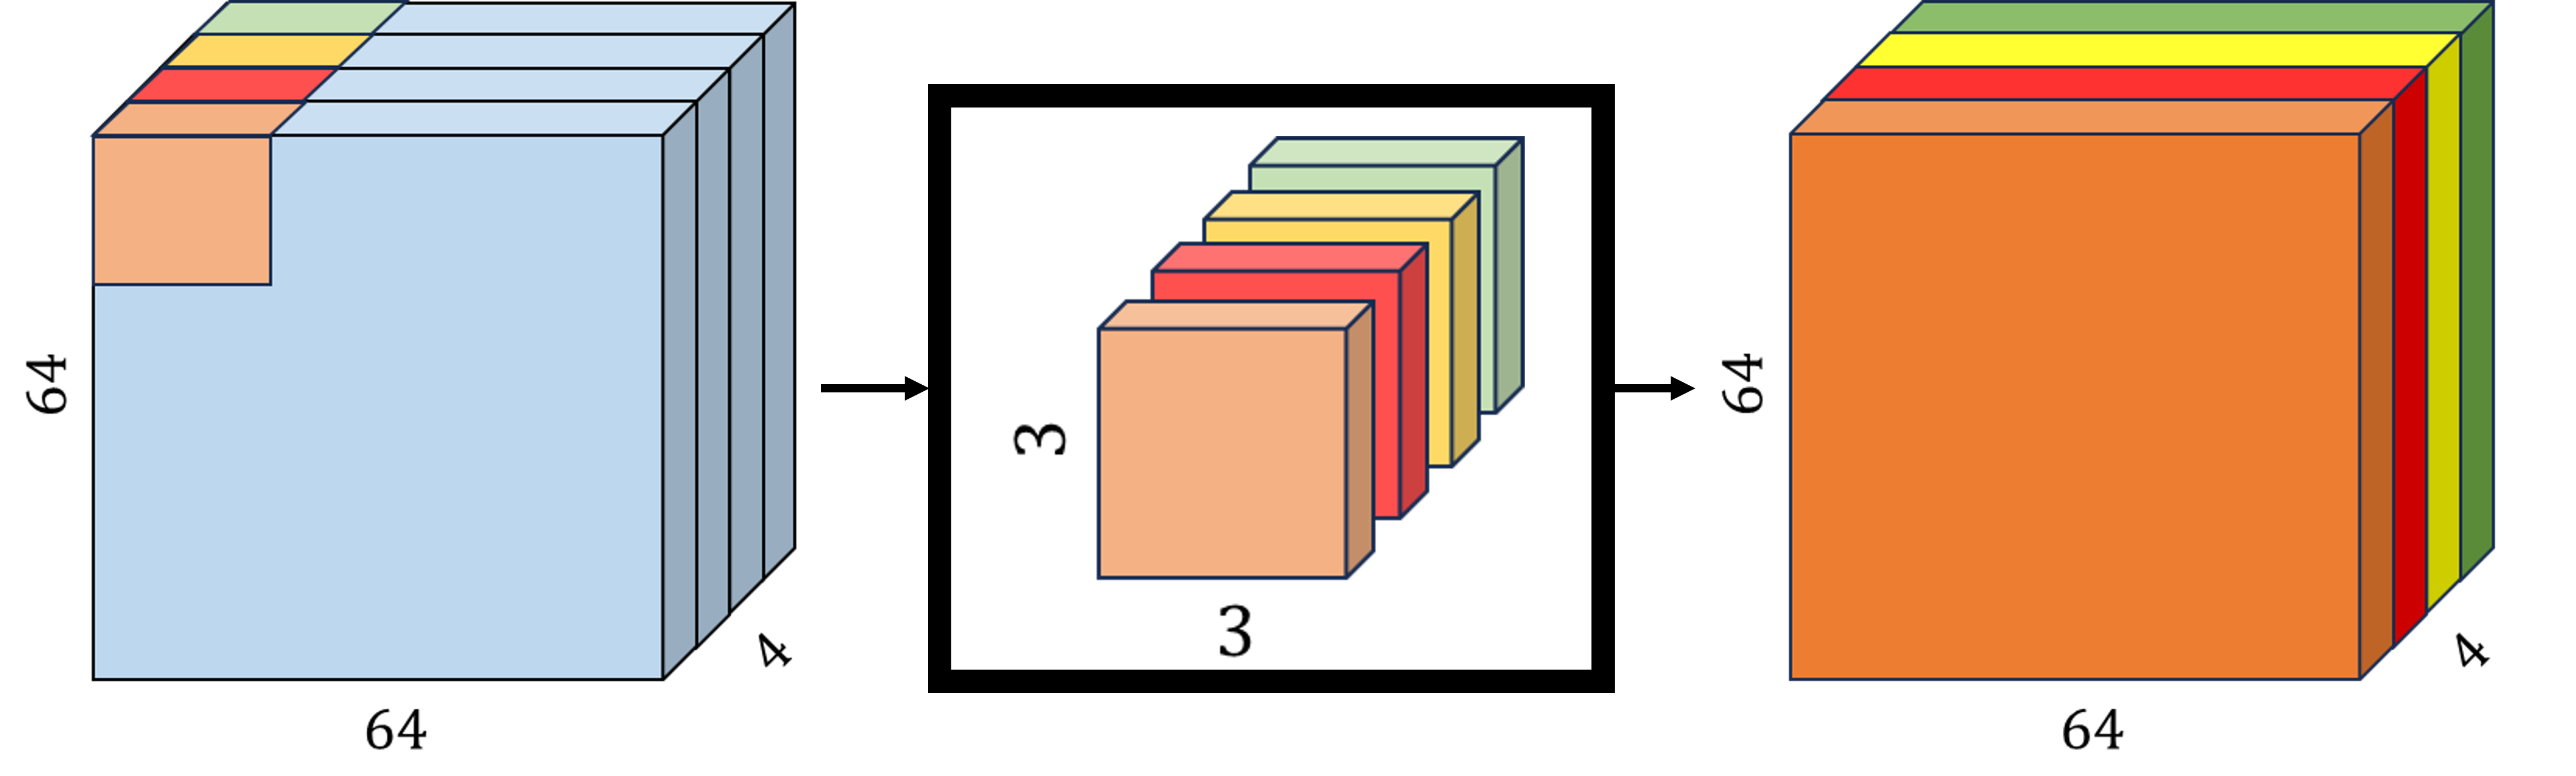
\includegraphics[width=12cm]{figures/sepconv.png}
    \caption{Schematic for a separable convolutional layer. Each channel is convolved with its own set of convolutional filters to obtain the best representation, as opposed to traditional convolutions where the same filter is applied to all channels in the data.}
    \label{sepconv}
\end{figure}

\begin{figure}[h]
    \centering
    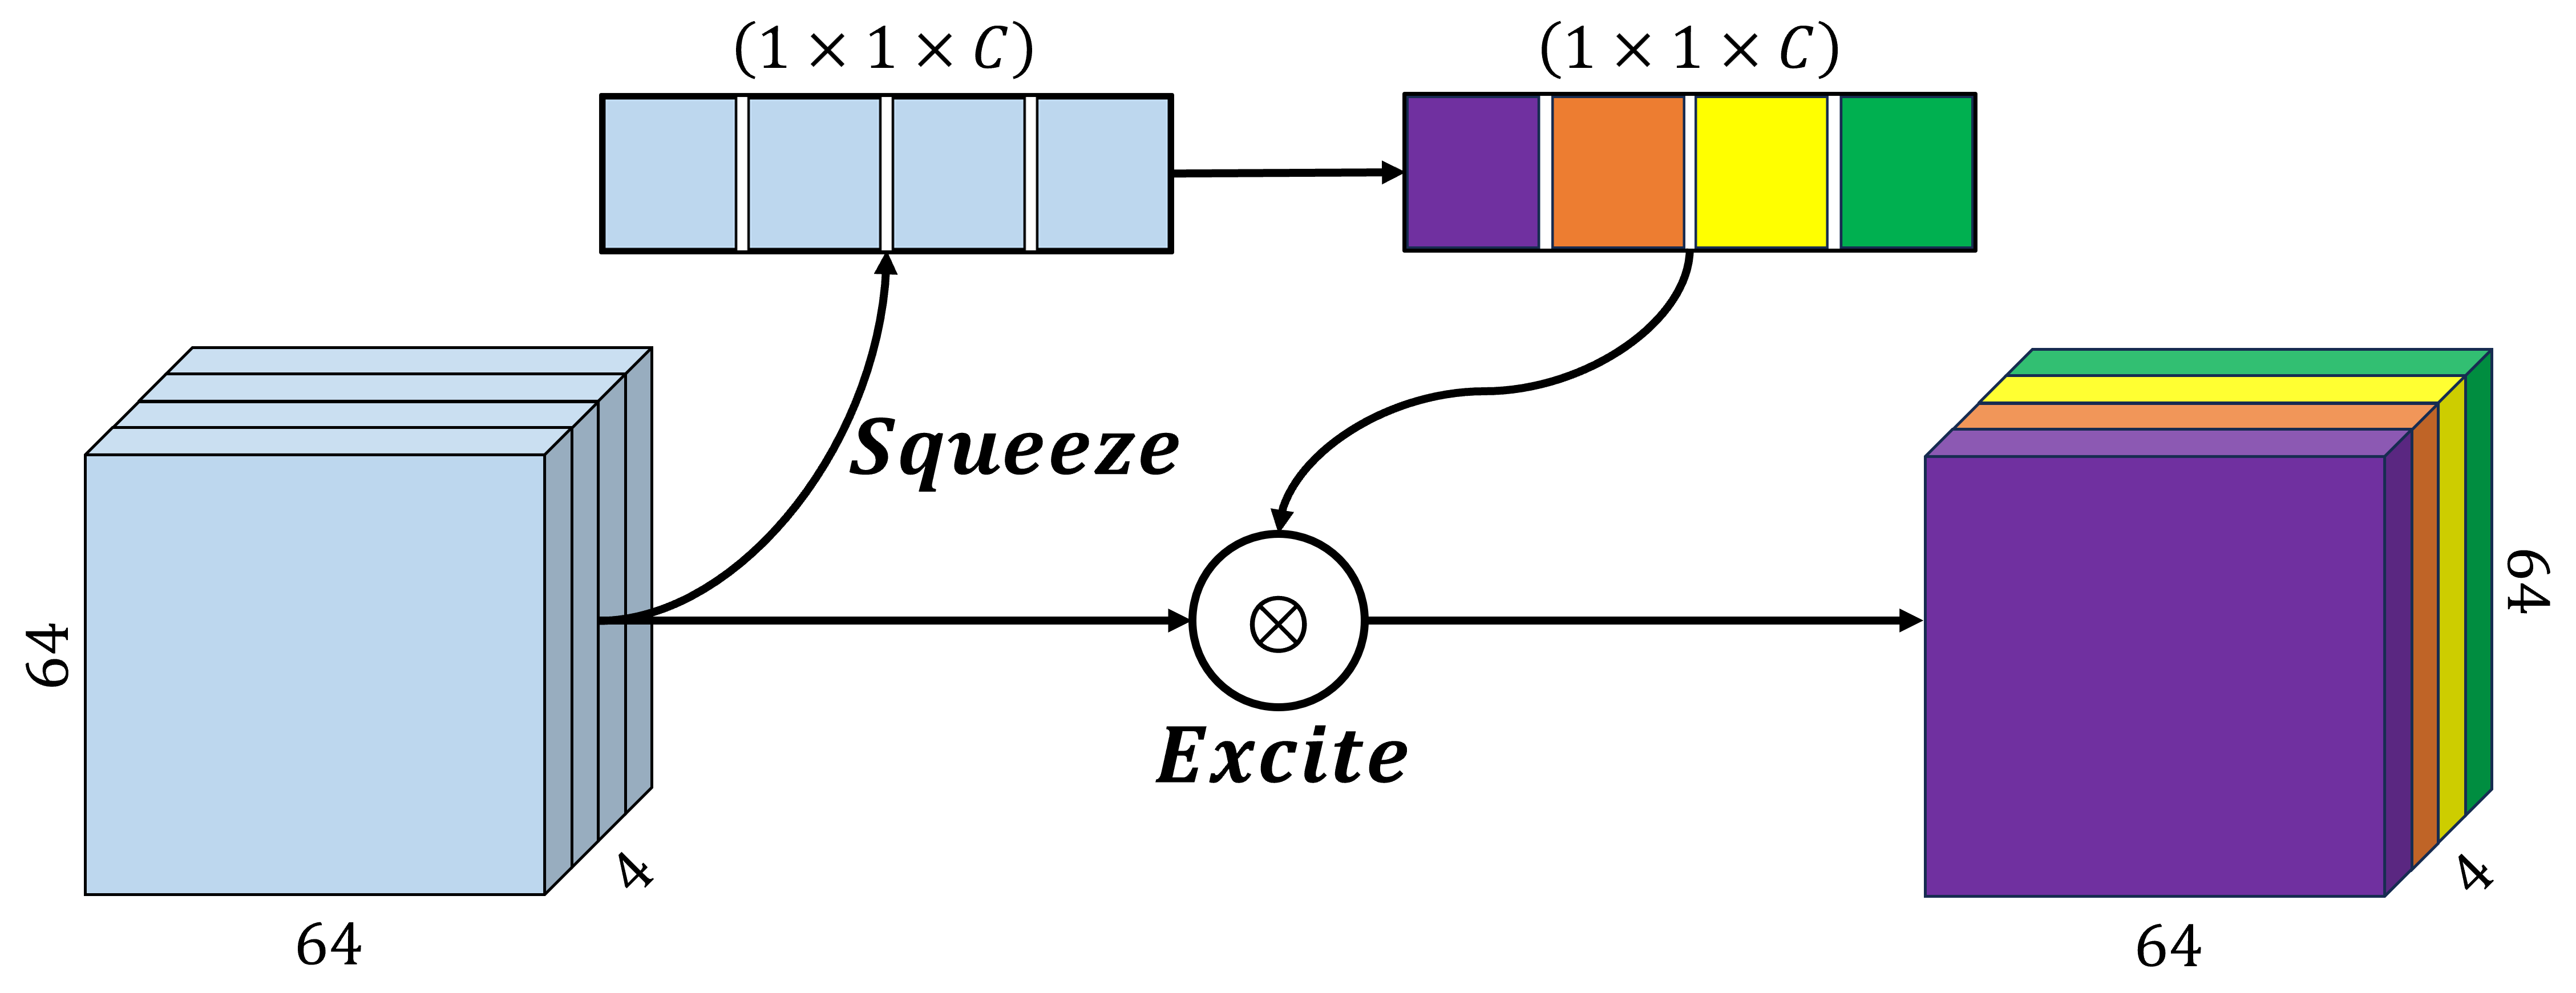
\includegraphics[width=12cm]{figures/squeeze-excite.png}
    \caption{Schematic for a squeeze-and-excite layer. The "squeeze" layer takes the global average of the data for each channel, and the "excite" layer is a fully-connected layer with nonlinear activation to estimate the optimal weights for each channel in the data. The result is a weighted representation of the data based on their intrinsic global characteristics.}
    \label{squeeze-excite}
\end{figure}

\begin{figure}[h]
    \centering
    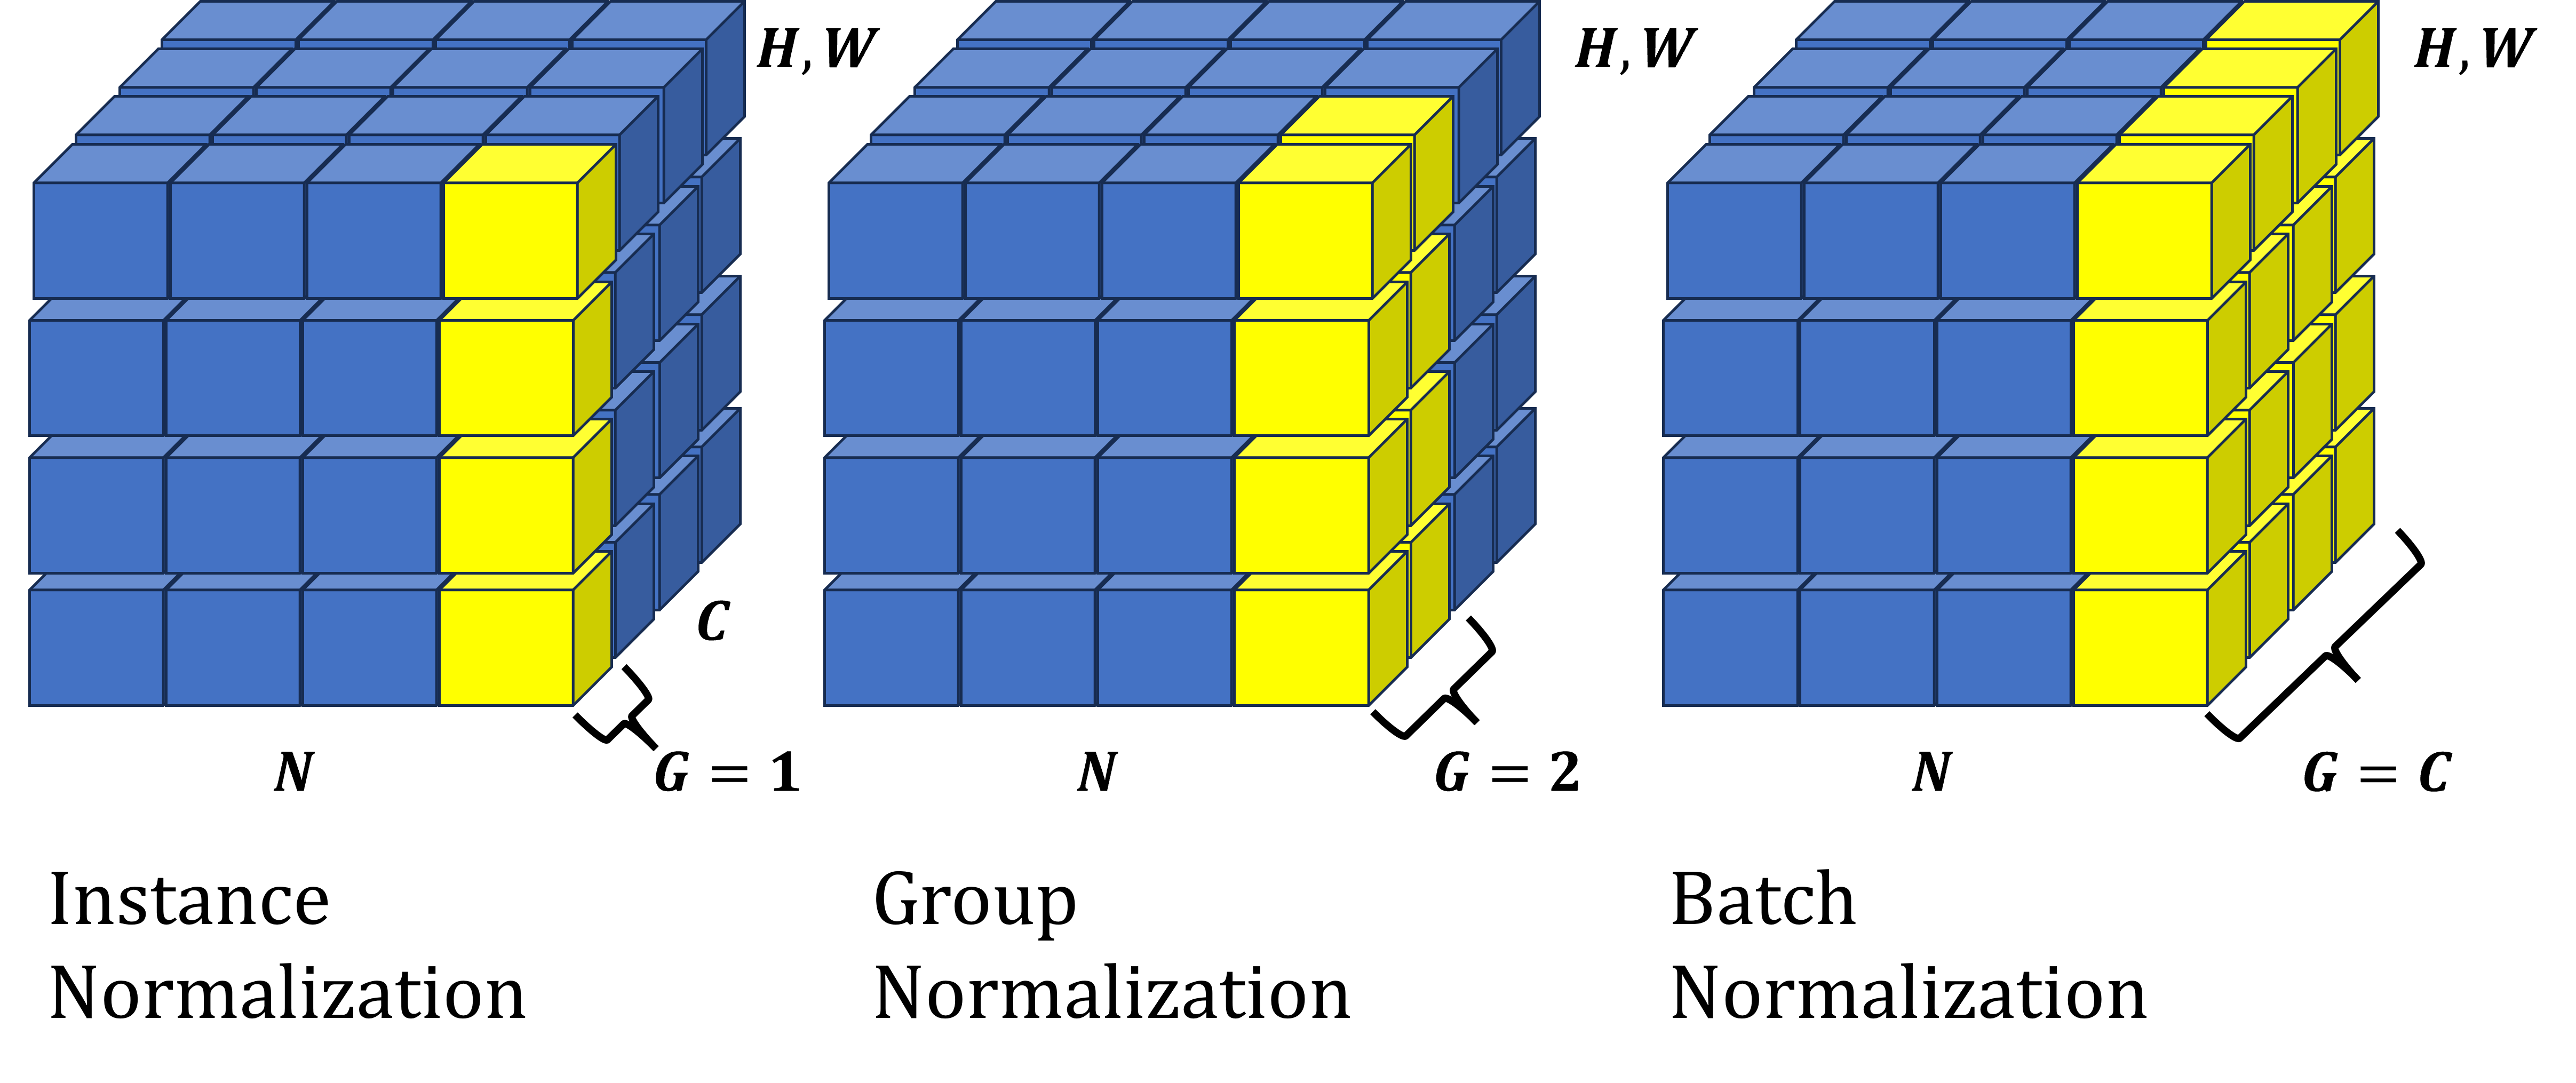
\includegraphics[width=12cm]{figures/instance-norm.png}
    \caption{Schematic for instance normalization (left) compared to group normalization (center) and batch normalization (right). In an instance normalization layer, each channel will be normalized by themselves rather than normalizing the entire batch or a subset of channels (groups).}
    \label{instance-norm}
\end{figure}

\begin{figure}[h]
    \centering
    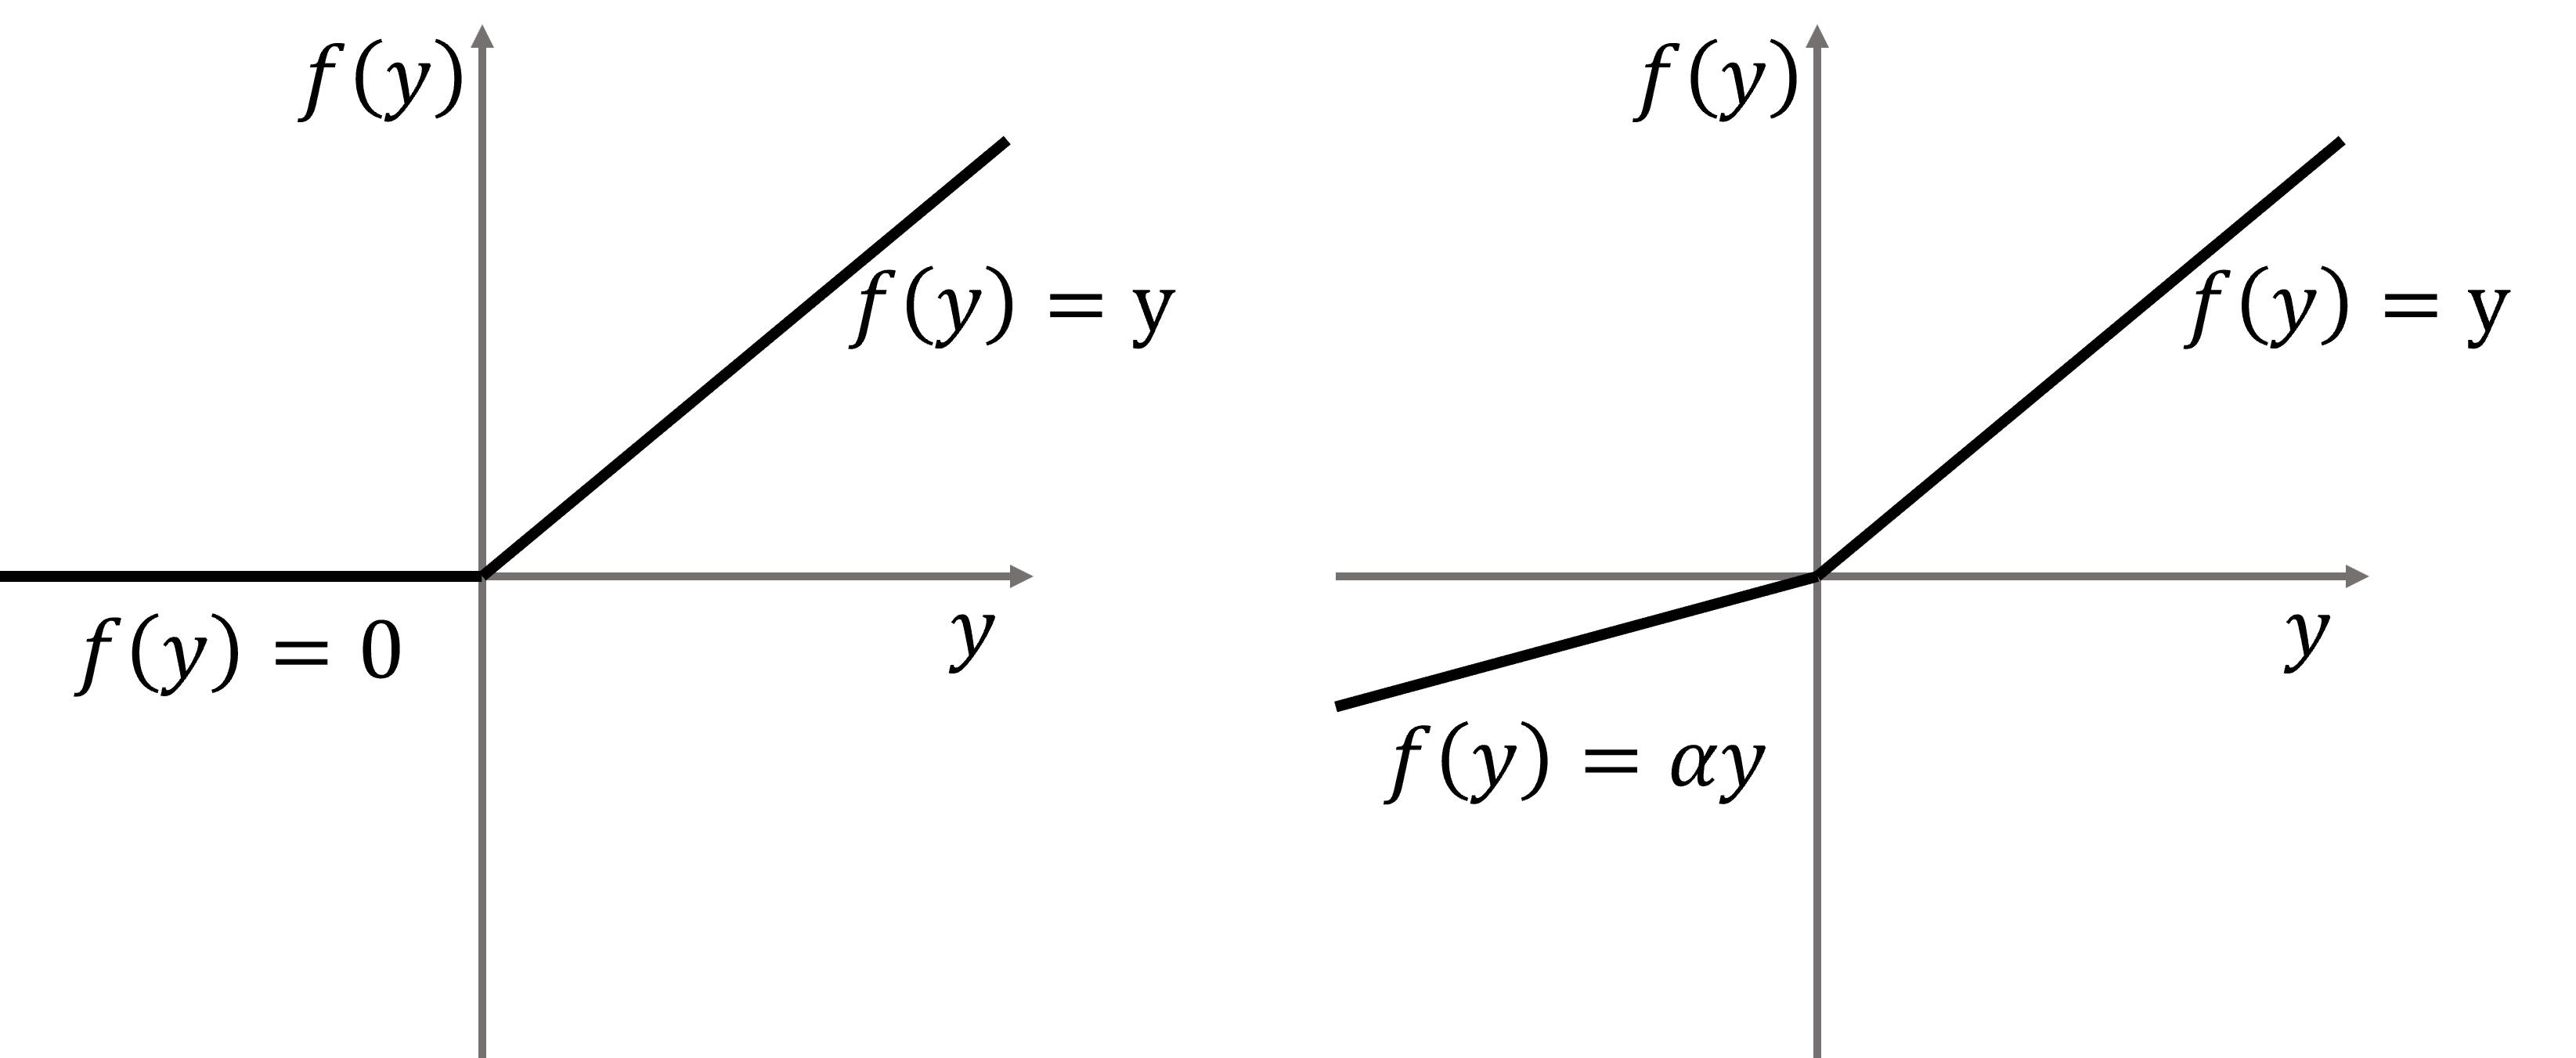
\includegraphics[width=10cm]{figures/prelu.png}
    \caption{Schematic for the Parametric Rectified Linear Unit (PReLU) activation function (right) compared to the traditional ReLU activation function (left). The slope of the negative portion of the data, $\alpha$, is learned for each batch.}
    \label{prelu}
\end{figure}

\begin{table*}[t]
    \caption{Encoder network architecture}\label{tab1}
    \centering
    \begin{tabular}{@{} llll @{} }
    \toprule
        \multirow{2}{*}{\textbf{Layer Number}} & \multirow{2}{*}{\textbf{Architecture}} & \textbf{Shape in} & \textbf{Shape out} \\
         &    & (h,w,c)   & (h,w,c)            \\
    \midrule
        \multirow{5}{*}{1} & SeparableConv2D    &  $64\times64\times4$ ($m$) & \\
                           & Squeeze-and-Excite &  &  \\
                           & Instance Norm      &  &  \\
                           & PReLU + Pooling    &  &  \\
                           & Spatial Dropout    &  & $32\times32\times64$ ($z_m^1$) \\
        \hline                      
        \multirow{5}{*}{2} & SeparableConv2D    & $32\times32\times64$ & \\
                           & Squeeze-and-Excite & & \\
                           & Instance Norm      & & \\
                           & PReLU + Pooling    & & \\
                           & Spatial Dropout    & & $16\times16\times128$ ($z_m^2$) \\
        \hline
        \multirow{5}{*}{3} & SeparableConv2D    & $16\times16\times128$ & \\
                           & Squeeze-and-Excite & & \\
                           & Instance Norm      & & \\
                           & PReLU + Pooling    & & \\
                           & Spatial Dropout    & & $8\times8\times256$  ($z_m^3$) \\
    \bottomrule
    \end{tabular}
\end{table*}

The decoder, $Dec^t(\cdot)$, of the Stochastic pix2vid model extracts the spatiotemporal relationships from the latent representations of $m$ to reconstruct the dynamic pressure and saturation distributions over time, $d$. To accurately reconstruct the spatiotemporal structure from the static latent space, $z_m$, we employ a series of convolutional-recurrent layers, namely a convolutional long-short term memory layer (ConvLSTM). The general form of a 2D ConvLSTM layer is shown in Figure \ref{convlstm}. Through 3 convolutional-recurrent layers, we obtain the dynamic prediction of $\hat{d}$ as follows:

\begin{enumerate}[Step 1:]\addtocounter{enumi}{5}
    \item \textbf{Spatiotemporal decoding of $z_m^3$}: The first ConvLSTM layer takes the smallest latent representation, $z_m^3$, and reconstructs the first decoded timestep $z_d^3$.
    
    \item \textbf{Residual concatenation of $z_m^2$}: The first decoded timestep, $z_d^3$, is concatenated with the intermediate static encoding $z_m^2$ to retain multi-scale features and improve prediction performance and resolution.
    
    \item \textbf{Intermediate spatiotemporal decoding}: The second ConvLSTM layer takes the residual concatenation of the intermediate latent representations, $[z_m^2,z_d^3]$, to predict the next spatiotemporal representation $z_d^2$. 
    
    \item \textbf{Residual concatenation of $z_m^1$}: The intermediate decoded timestep, $z_d^2$, is concatenated with the largest static encoding $z_m^1$.
    
    \item \textbf{Final spatiotemporal decoding}: The third ConvLSTM layer takes the residual concatenation of the larger latent representations, $[z_m^1,z_d^2]$, to predict the full-scale dynamic output, $d$.
\end{enumerate}

\begin{figure}[h]
    \centering
    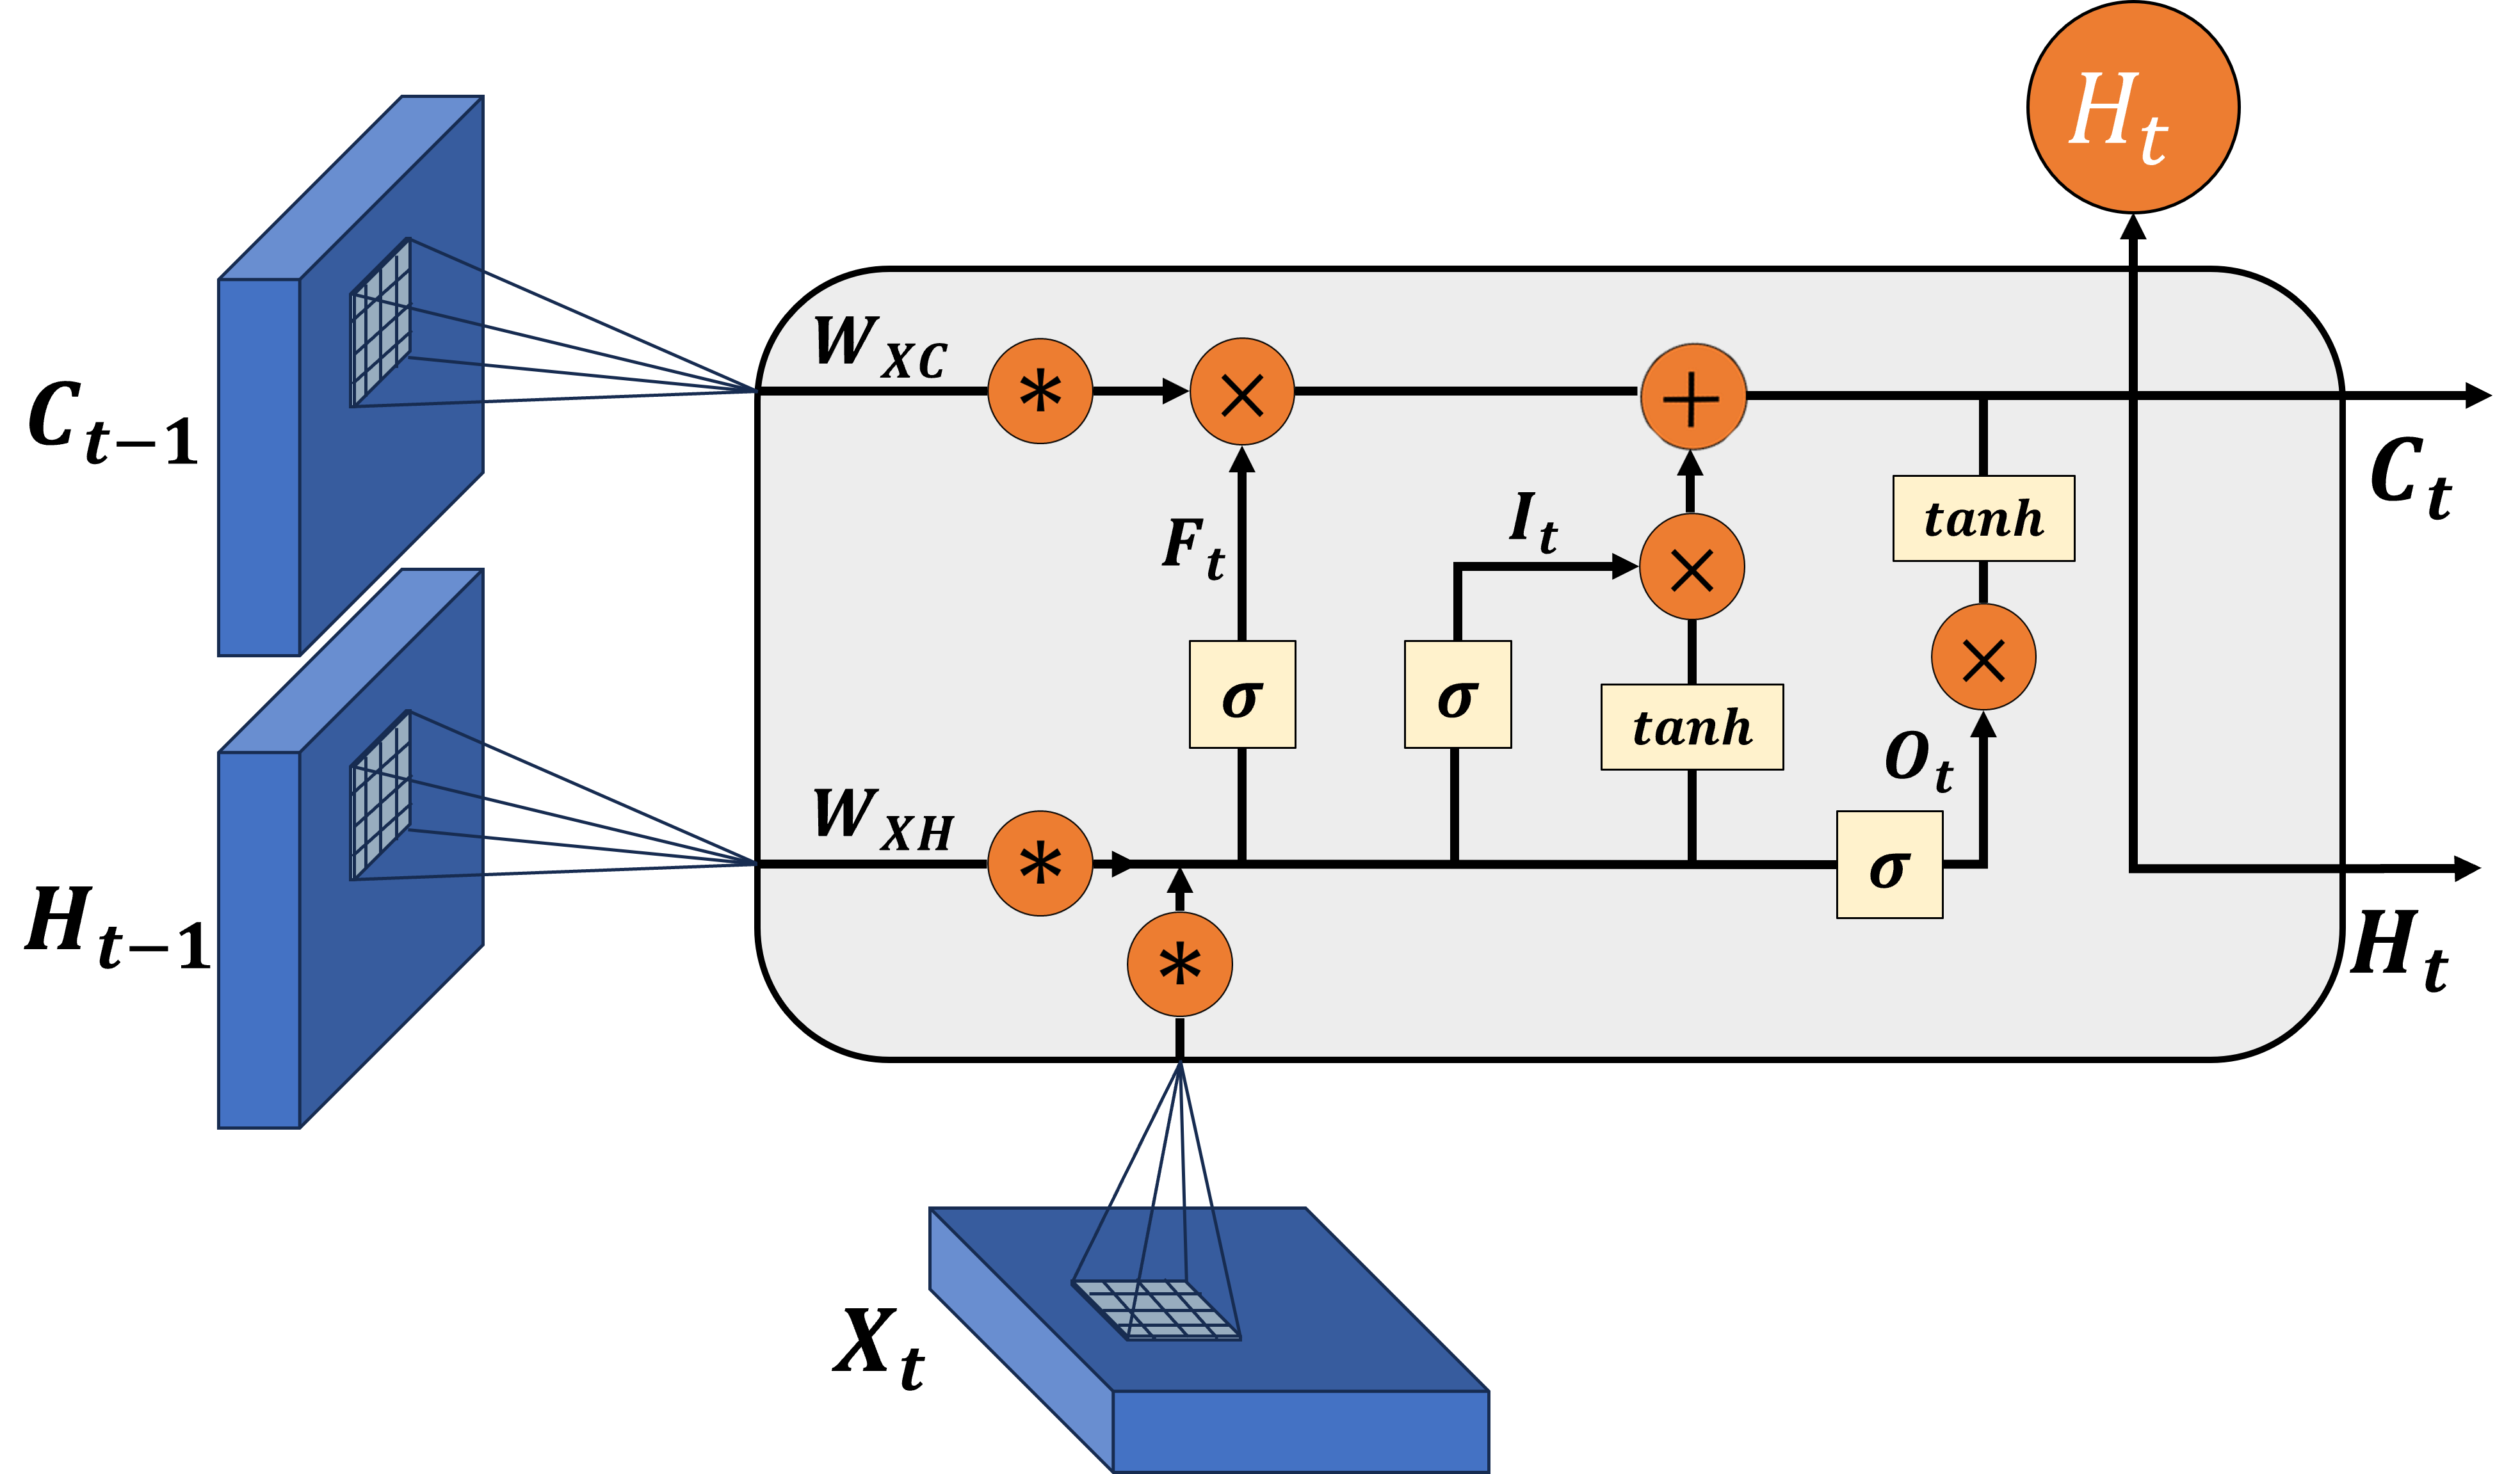
\includegraphics[width=12cm]{figures/convlstm.png}
    \caption{Schematic of a convolutional-LSTM (ConvLSTM) layer. The layer applies convolutional operations to the input data using a set of learnable filters to capture the spatial patterns. The recurrent part is a long short-term memory layer with memory and forget gates to capture the temporal patterns. LSTM units are applied to each spatial location separately allowing to capture both spatial and temporal dependencies in the data.}
    \label{convlstm}
\end{figure}

To enhance the performance of the spatiotemporal decoding, each ConvLSTM layer is followed by a batch normalization, activation, and a transpose convolutional layer, the latter for downscaling the latent features to twice their dimension. Spatial dropout is applied, and the concatenated features are once more convolved and activated to obtain the layer prediction. Table \ref{tab2} shows the architecture of the decoder network.

\begin{table*}[t]
    \caption{Decoder network architecture}\label{tab2}
    \centering
    \begin{tabular}{@{} llll @{} }
    \toprule
        \multirow{2}{*}{\textbf{Layer Number}} & \multirow{2}{*}{\textbf{Architecture}} &
        \textbf{Shape in} & \textbf{Shape out} \\ & & (t,h,w,c) & (t,h,w,c) \\
    \midrule
        \multirow{6}{*}{1} & ConvLSTM2D & $1\times8\times8\times256$ & \\
                           & BatchNorm + LeakyReLU & & \\
                           & Conv2DTranspose       & & \\
                           & Spatial Dropout       & & \\
                           & Concatenate ($z_m^3$) & & \\
                           & Conv2D + Sigmoid      & & $t\times16\times16\times128$ ($z_{d_t}^3$) \\
        \hline                      
        \multirow{6}{*}{2} & ConvLSTM2D & $t\times16\times16\times128$ & \\
                           & BatchNorm + LeakyReLU & & \\
                           & Conv2DTranspose       & & \\
                           & Spatial Dropout       & & \\
                           & Concatenate ($z_m^2$) & & \\
                           & Conv2D + Sigmoid      & & $t\times32\times32\times64$ ($z_{d_t}^2$) \\
        \hline
        \multirow{6}{*}{3} & ConvLSTM2D & $t\times32\times32\times64$ & \\
                           & BatchNorm + LeakyReLU & & \\
                           & Conv2DTranspose       & & \\
                           & Spatial Dropout       & & \\
                           & Concatenate ($z_m^1$) & & \\
                           & Conv2D + Sigmoid      & & $t\times64\times64\times2$ ($z_{d_t}^1$) \\
    \bottomrule
    \end{tabular}
\end{table*}

This process yields the first video frame prediction, $d_1$, from the latent representation of the geologic realizations $z_m$. Each subsequent video frame prediction is obtained by another set of residual concatenation of the previous timestep dynamic decoded representation. The static latent representation $z_m$ is concatenated at each timestep with the previous dynamic decoded representation for each layer such that we have $[z_m,z_{d_t}^i]$, where $i$ is the decoding layer number and $t$ is the timestep. By recursively implementing spatiotemporal decoding to the latent representation $z_m$, we obtain the prediction of the dynamic response $d_t$ at times for each timestep $t=1,\ldots,n$.

The complete Stochastic pix2vid architecture is shown in Figure \ref{cnnrnn_architecture}. Here we observe the spatial compression of the geologic models, $m$, through the encoding portion of the network, and the spatiotemporal decoding and residual multi-scale concatenations through the decoder portion of the network. The resulting architecture provides proxy model from a subsurface static uncertainty model (images) to subsurface dynamic response (videos).

\begin{figure*}[t]
    \centering
    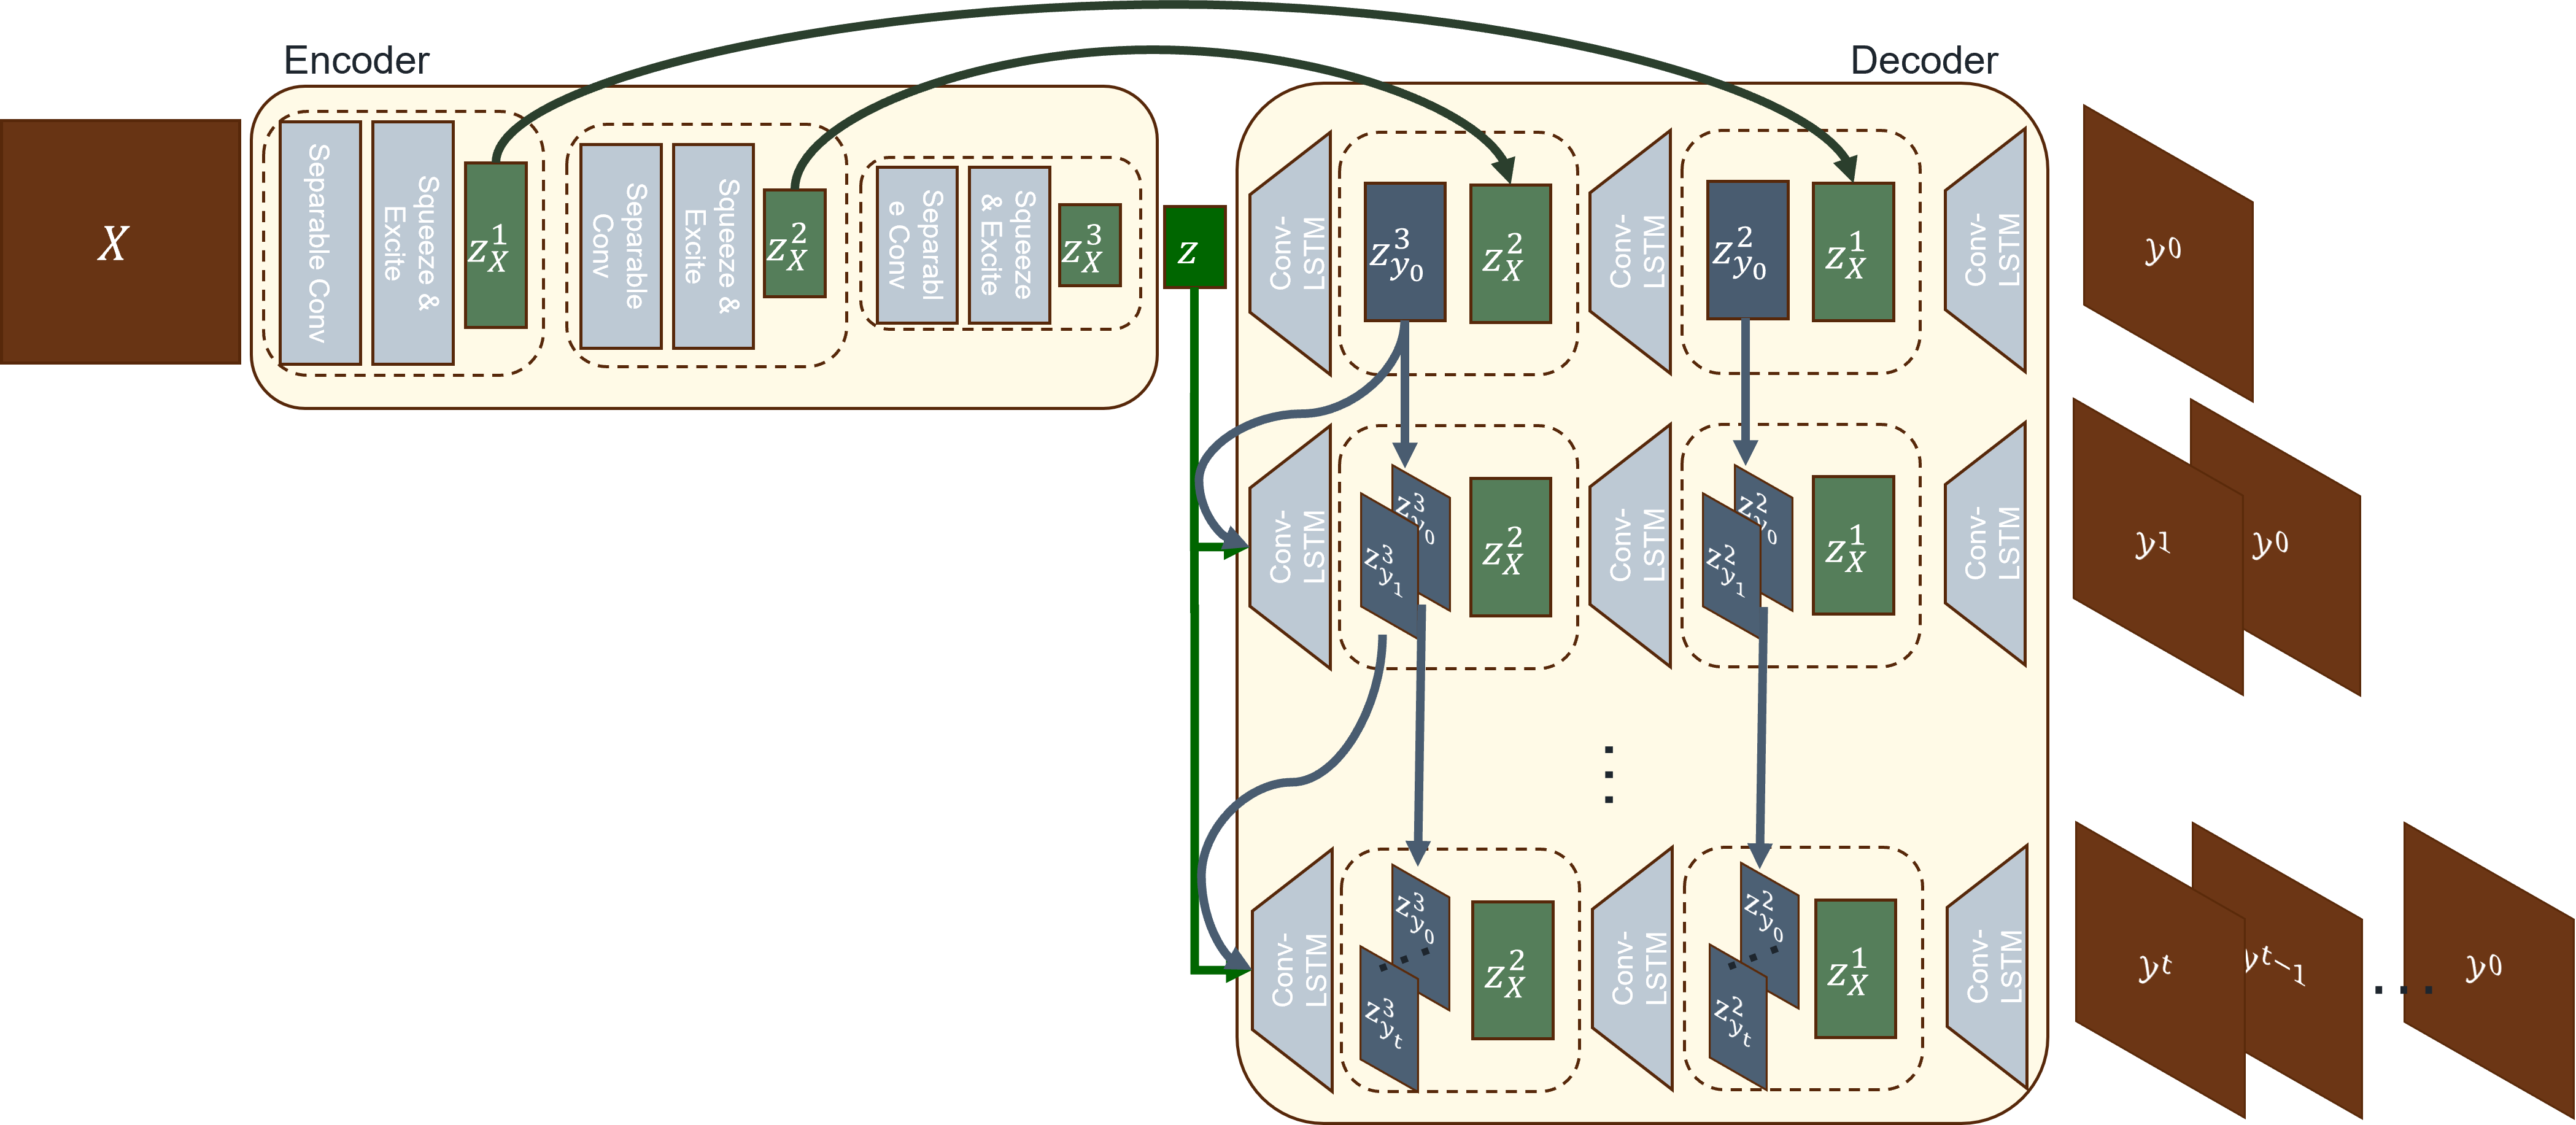
\includegraphics[width=\textwidth]{figures/architecture.png}
    \caption{Architecture of our proposed Stochastic pix2vid method. The input data, $X\equiv m$, is encoded through a series of convolutional layers to capture the spatial dependencies in the geologic models. The latent representation, $z_m$, is recursively passed through a spatiotemporal decoder with convolutional-recurrent layers, and concatenated with the residuals of the encoder to reconstruct iteratively the frames of the output (video) data, $y\equiv d$.}
    \label{cnnrnn_architecture}
\end{figure*}


%%========= subsection 2.3 =========%%
\textbf{2.3 Training Strategy} 

The inputs to the Stochastic pix2vid are the geologic realizations, comprised of the distributions of porosity, permeability, facies, and injection well(s) location, represented as a matrix $m$ of dimensions $64\times64\times4$. The outputs are the results from the numerical reservoir simulation, namely pressure and saturation distributions over time, represented as a matrix $d$ of dimensions $64\times64\times60\times2$. This yields an ill-posed and under-determined estimation problem, which are difficult to resolve \cite{tarantola2005inverse, Oliver20081}. To improve the training efficiency and performance, we subsample in time from 60 timesteps to 11. In other words, instead of monthly monitoring, we predict the dynamic outputs at the initial step and every 6 months afterward; therefore the output matrices, $(d, \hat{d})$, have a final dimension of $64\times64\times11\times2$. This is done to make the problem more tractable and speed up the training and prediction process, while retaining majority of the temporal information. 

We also perform min-max normalization so that the input and output features are in the range of $[0,1]$, which greatly improves the performance of the nonlinear activation functions. Furthermore, we perform data augmentation by $90^{\circ}$ image rotation, making the network agnostic to orientation and encourage effectively learning the flow physics in the system rather than memorizing spatial distribution patterns. The total amount of training data is therefore 2,000 realizations (after augmentation), which is split into 1,500 realizations for training and 500 realizations for testing. To improve model generalizability, at each epoch, each training set minibatch is further split into a training and validation subset using an 80/20 split. The validation set is only used to adjust the trainable model parameters for each batch at each epoch and is randomly partitioned from the training batch at every epoch, while the testing data remains unseen to quantify the model performance after training.

A custom three-part loss function is used to accurately predict pixel-wise and perceptual information in the predictions. The mean squared error (MSE) is used to reconstruct the pixel-wise intensity values, while the mean absolute error (MAE) is used to optimize for the pressure and saturation plume edges. The third part is the structural similarity index metric (SSIM), which provides a perceptual image-to-image comparison of luminance, contrast, and structure \cite{Bovik2004}. For optimal training, the aim is to minimize the MSE and MAE while maximizing the SSIM for the true versus predicted outputs, $d$ and $\hat{d}$, such that the total loss is given by $\mathcal{L} = \alpha(1-SSIM) + (1-\alpha)[\beta MSE + (1-\beta) MAE] $, where $\alpha$ and $\beta$ are weighting coefficients obtained empirically as 0.33 and 0.66, respectively.

The model is trained using the AdamW optimizer \cite{loshchilov2017decoupled}. This variant of the well-known adaptive momentum (Adam) optimizer \cite{kingma2014adam} includes an added method to decay weights for the adaptive estimation of first-order and second-order moments. We implement a learning rate of $1\times10^{-3}$ with a weight decay term of $1\times10^{-5}$. 


%%==================================%%
%%              RESULTS             %%
%%==================================%%
\section*{\textbf{3 Results}}

This section describes the geologic model generation, training performance and discusses the application of the Stochastic pix2vid proxy to rapidly forecast CO$_2$ plume migration for a large-scale GCS operation.

%%========= subsection 3.1 =========%%
\textbf{3.1 Reservoir Model and Simulation}

We use SGeMS \cite{Remy2009} to construct the subsurface uncertainty model, an ensemble of static feature realiations that is representative of various potential geologic scenarios for CO$_2$ storage. Using sequential Gaussian co-simulation \cite{Verly1993}, we generate a set of 1,000 random porosity ($\phi$) and permeability ($k$) distributions with a wide range of values, as shown in Figure \ref{geomodels}. Facies distributions are obtained from a library of deepwater fluvial training images \cite{PYRCZ2008542, misael_m_morales_2023_7702128}. These encompass a wide range of possible geologic scenarios including marked point (lobe, ellipse, and bar), FluvSim (channel, channel-levee, and channel-levee-splay), surface based (compensational cycles of lobes), and bank retreat (channel complex). To generate consistent porosity and permeability distributions with the facies-based geologic scenarios, we condition the original porosity and permeability distributions to the facies distributions. The resulting fluvial distributions are shown in Figure \ref{conditioned_geomodels}. 

\begin{figure*}[t]
    \centering
    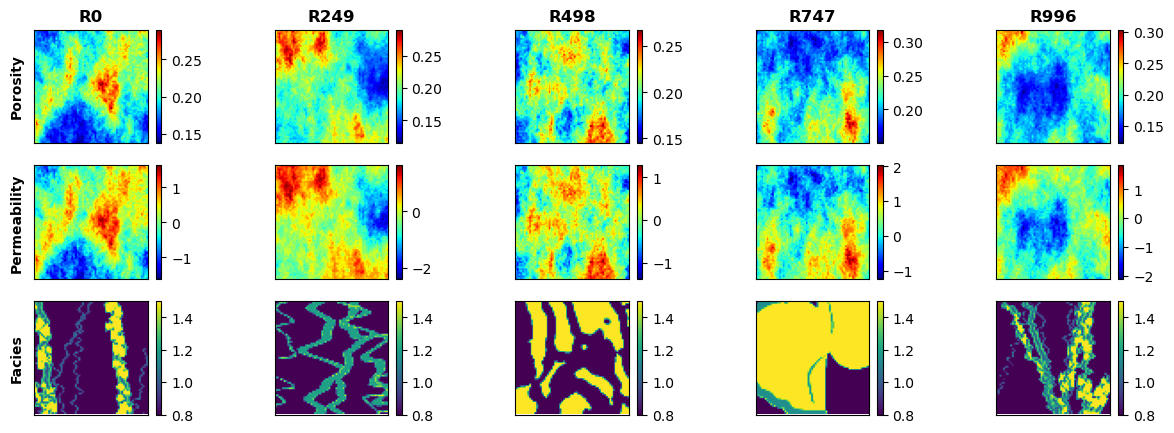
\includegraphics[width=\textwidth]{figures/geomodels.png}
    \caption{Spatial distribution of porosity (top), permeability (middle), and facies (bottom) for 5 random realizations.}
    \label{geomodels}
\end{figure*}

\begin{figure*}[t]
    \centering
    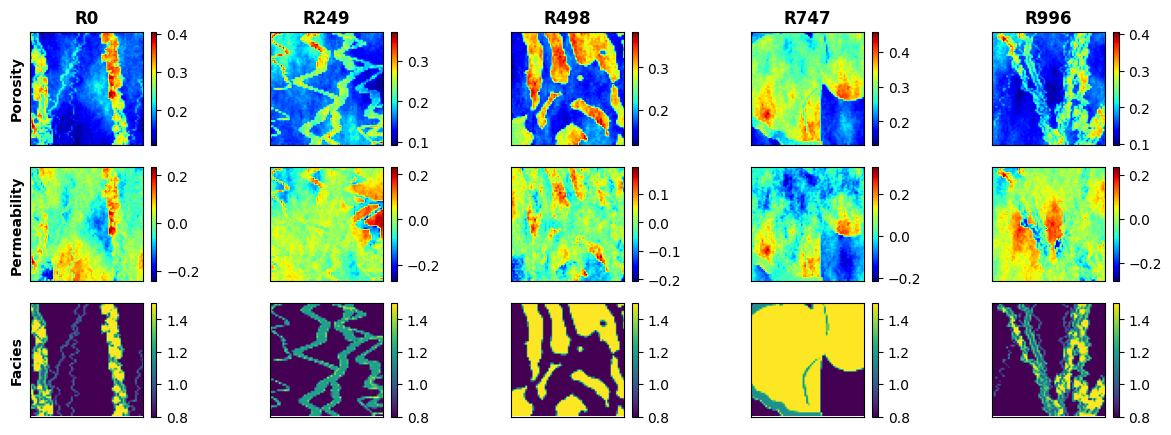
\includegraphics[width=\textwidth]{figures/conditioned_geomodels.png}
    \caption{Spatial distribution conditioned to facies (top) for porosity (middle) and permeability (bottom) for 5 random realizations.}
    \label{conditioned_geomodels}
\end{figure*}

The model has dimensions of 1km-1km-100m in the x-, y-, and z-directions, respectively. We use 64 uniform grid cells in the x- and y-directions. The grid design is sufficiently refined to resolve the pressure and saturation plumes in highly heterogeneous reservoirs while remaining computationally tractable for the purpose of training deep learning models. A random number of injection wells, $w \in [1,3]$, are placed randomly along the reservoir for each of the 1,000 realizations, no closer than 250m from the boundaries, as shown in Figure \ref{wells_dist}. The injection well(s) are randomly placed and not conditioned to zones of preferential porosity, permeability, nor facies. Each injection well has a constant radius of 0.1m and a single and continuous perforation that injects pure supercritical CO$_2$ at a constant rate such that the total injection rate of the $w$ well(s) is 0.5 megatons per year.

\begin{figure*}[t]
    \centering
    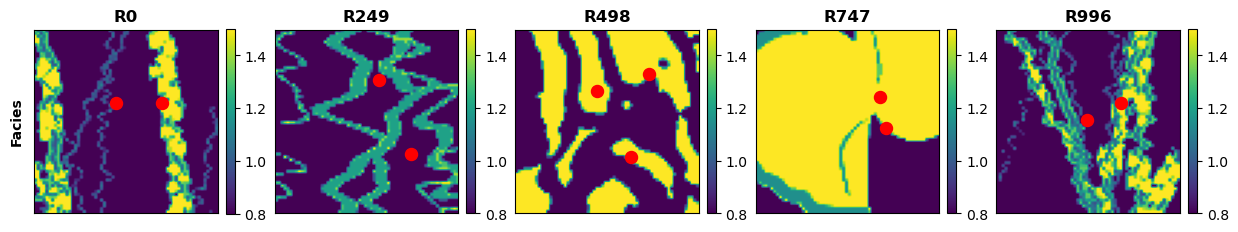
\includegraphics[width=\textwidth]{figures/wells_dist.png}
    \caption{CO$_2$ injection well(s) location (red) overlaid over facies distributions for 5 random realizations.}
    \label{wells_dist}
\end{figure*}

The conditional fluvial porosity and permeability distributions are used as input models for the numerical simulation of geologic CO$_2$ storage using MRST \cite{MRST2019} to calculate the response models for training our proposed model. The reservoir is initialized as a fully water saturated zone (i.e., aquifer) with an initial pressure of 4,000 psi. The reservoir has constant isothermal conditions and constant pressure boundary conditions to represents a large-scale geologic CO$_2$ storage project with negligible dip, such as found in the Illinois Basin and parts of the North Sea and Gulf of Mexico. 

The numerical simulation is run for 5 years, monitored monthly, for a total of 60 timesteps. At each grid cell and for each time step, we resolve the implicit pressure, explicit saturation (IMPES) formulation of Eq. \eqref{eq1} to obtain the corresponding dynamic pressure and saturation distributions over time (videos) from the static geologic realizations of porosity and permeability conditioned to the fluvial facies (images) with random well(s) configuration. The pressure and saturation responses corresponding to the geologic model realizations are shown in Figures \ref{pres_response} and \ref{sat_response}, respectively.

\begin{figure*}[t]
    \centering
    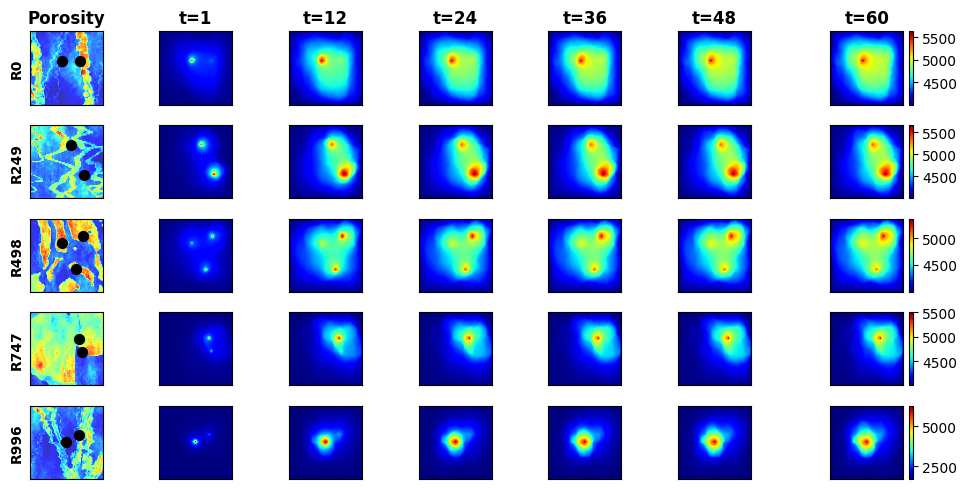
\includegraphics[width=\textwidth]{figures/pres_response.png}
    \caption{Pressure response distributions over time (in psia) obtained by HFS for the 5 random realizations from Fig. \ref{conditioned_geomodels}.}
    \label{pres_response}
\end{figure*}

\begin{figure*}[t]
    \centering
    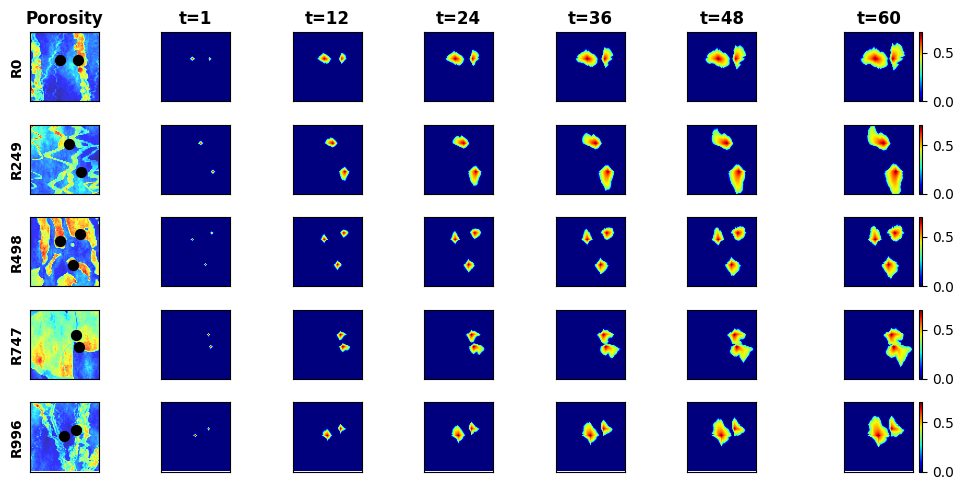
\includegraphics[width=\textwidth]{figures/sat_response.png}
    \caption{Saturation response distributions over time obtained by HFS for the 5 random realizations obtained from Fig. \ref{conditioned_geomodels}.}
    \label{sat_response}
\end{figure*}

%%========= subsection 3.2 =========%%
\textbf{3.2 Training Performance}

Using an NVIDIA Quadro M6000 GPU, we train for 100 epochs with batch size of 50. The model has in total 97,523,370 parameters, and the training time required is approximately 88 minutes for all 1,500 training realizations. The training and validation performance per epoch is shown in Figure \ref{train_perf}. We observe minimal overfit in the validation set, corresponding to good model generalizability and prediction accuracy within the training data. Using physics-based numerical simulation, each realization requires approximately 30 seconds to obtain the dynamic pressure and saturation predictions from the static geologic models. Our Stochastic pix2vid model obtains the same results in approximately 4.59 milliseconds, corresponding to a 6,500× speedup. The average MSE for the ensemble is $9.21\times10^{-4}$ and $9.70\times10^{-4}$ for training and testing, respectively. Similarly, the average SSIM for the ensemble is $98.97\%$ and $97.91\%$ for training and testing, respectively.

\begin{figure}[h]
    \centering
    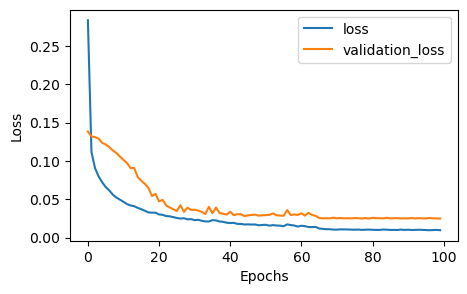
\includegraphics[width=7.5cm]{figures/train_performance.png}
    \caption{The total training and validation losses, $\mathcal{L}$, as a function of epoch number.}
    \label{train_perf}
\end{figure}

%%========= subsection 3.3 =========%%
\textbf{3.3 Prediction Results}

After training the Stochastic pix2vid model with 1,500 realizations of static geologic models, $m=\{\phi,k,facies,w\}$, to predict the dynamic reservoir response, $d=\{P(t),S(t)\}$, we can compare the performance of the predictions for the training and unseen testing data. 

Figures \ref{train_pres} and \ref{train_sat} show the predicted dynamic pressure and saturation distributions, respectively, along with the absolute difference to HFS for 3 training realizations. We observe reasonable agreement between the true and predicted CO$_2$ pressure and saturation plumes over time, pixel-wise with an average MSE of $3.25\times10^{-4}$ and perceptually with SSIM of $98.59\%$ for pressure predictions and MSE of $1.50\times10^{-4}$ and SSIM of $97.31\%$ for saturation predictions.

\begin{figure}
    \centering
    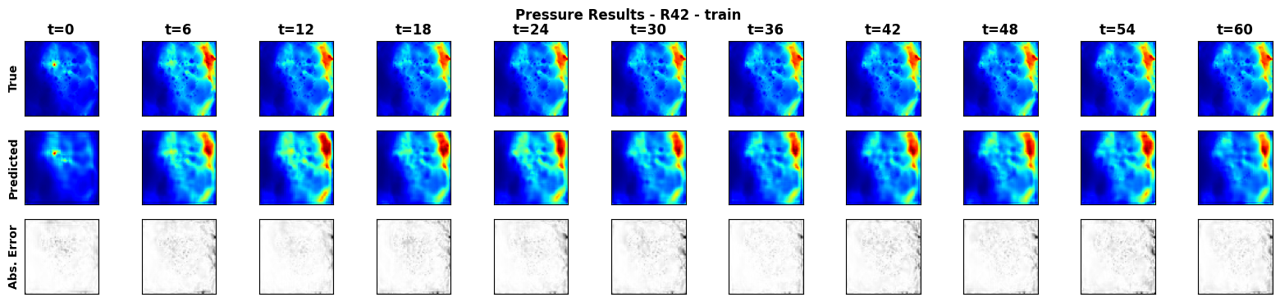
\includegraphics[width=\textwidth,height=0.95\textheight,keepaspectratio]{figures/train_pres.png}
    \caption{Normalized pressure distribution over time for 3 random training realization. For each panel, the top row is the ground truth from the HFS, the middle row is the Stochastic pix2vid prediction, and the bottom row is the absolute difference to HFS.}
    \label{train_pres}
\end{figure}

\begin{figure}
    \centering
    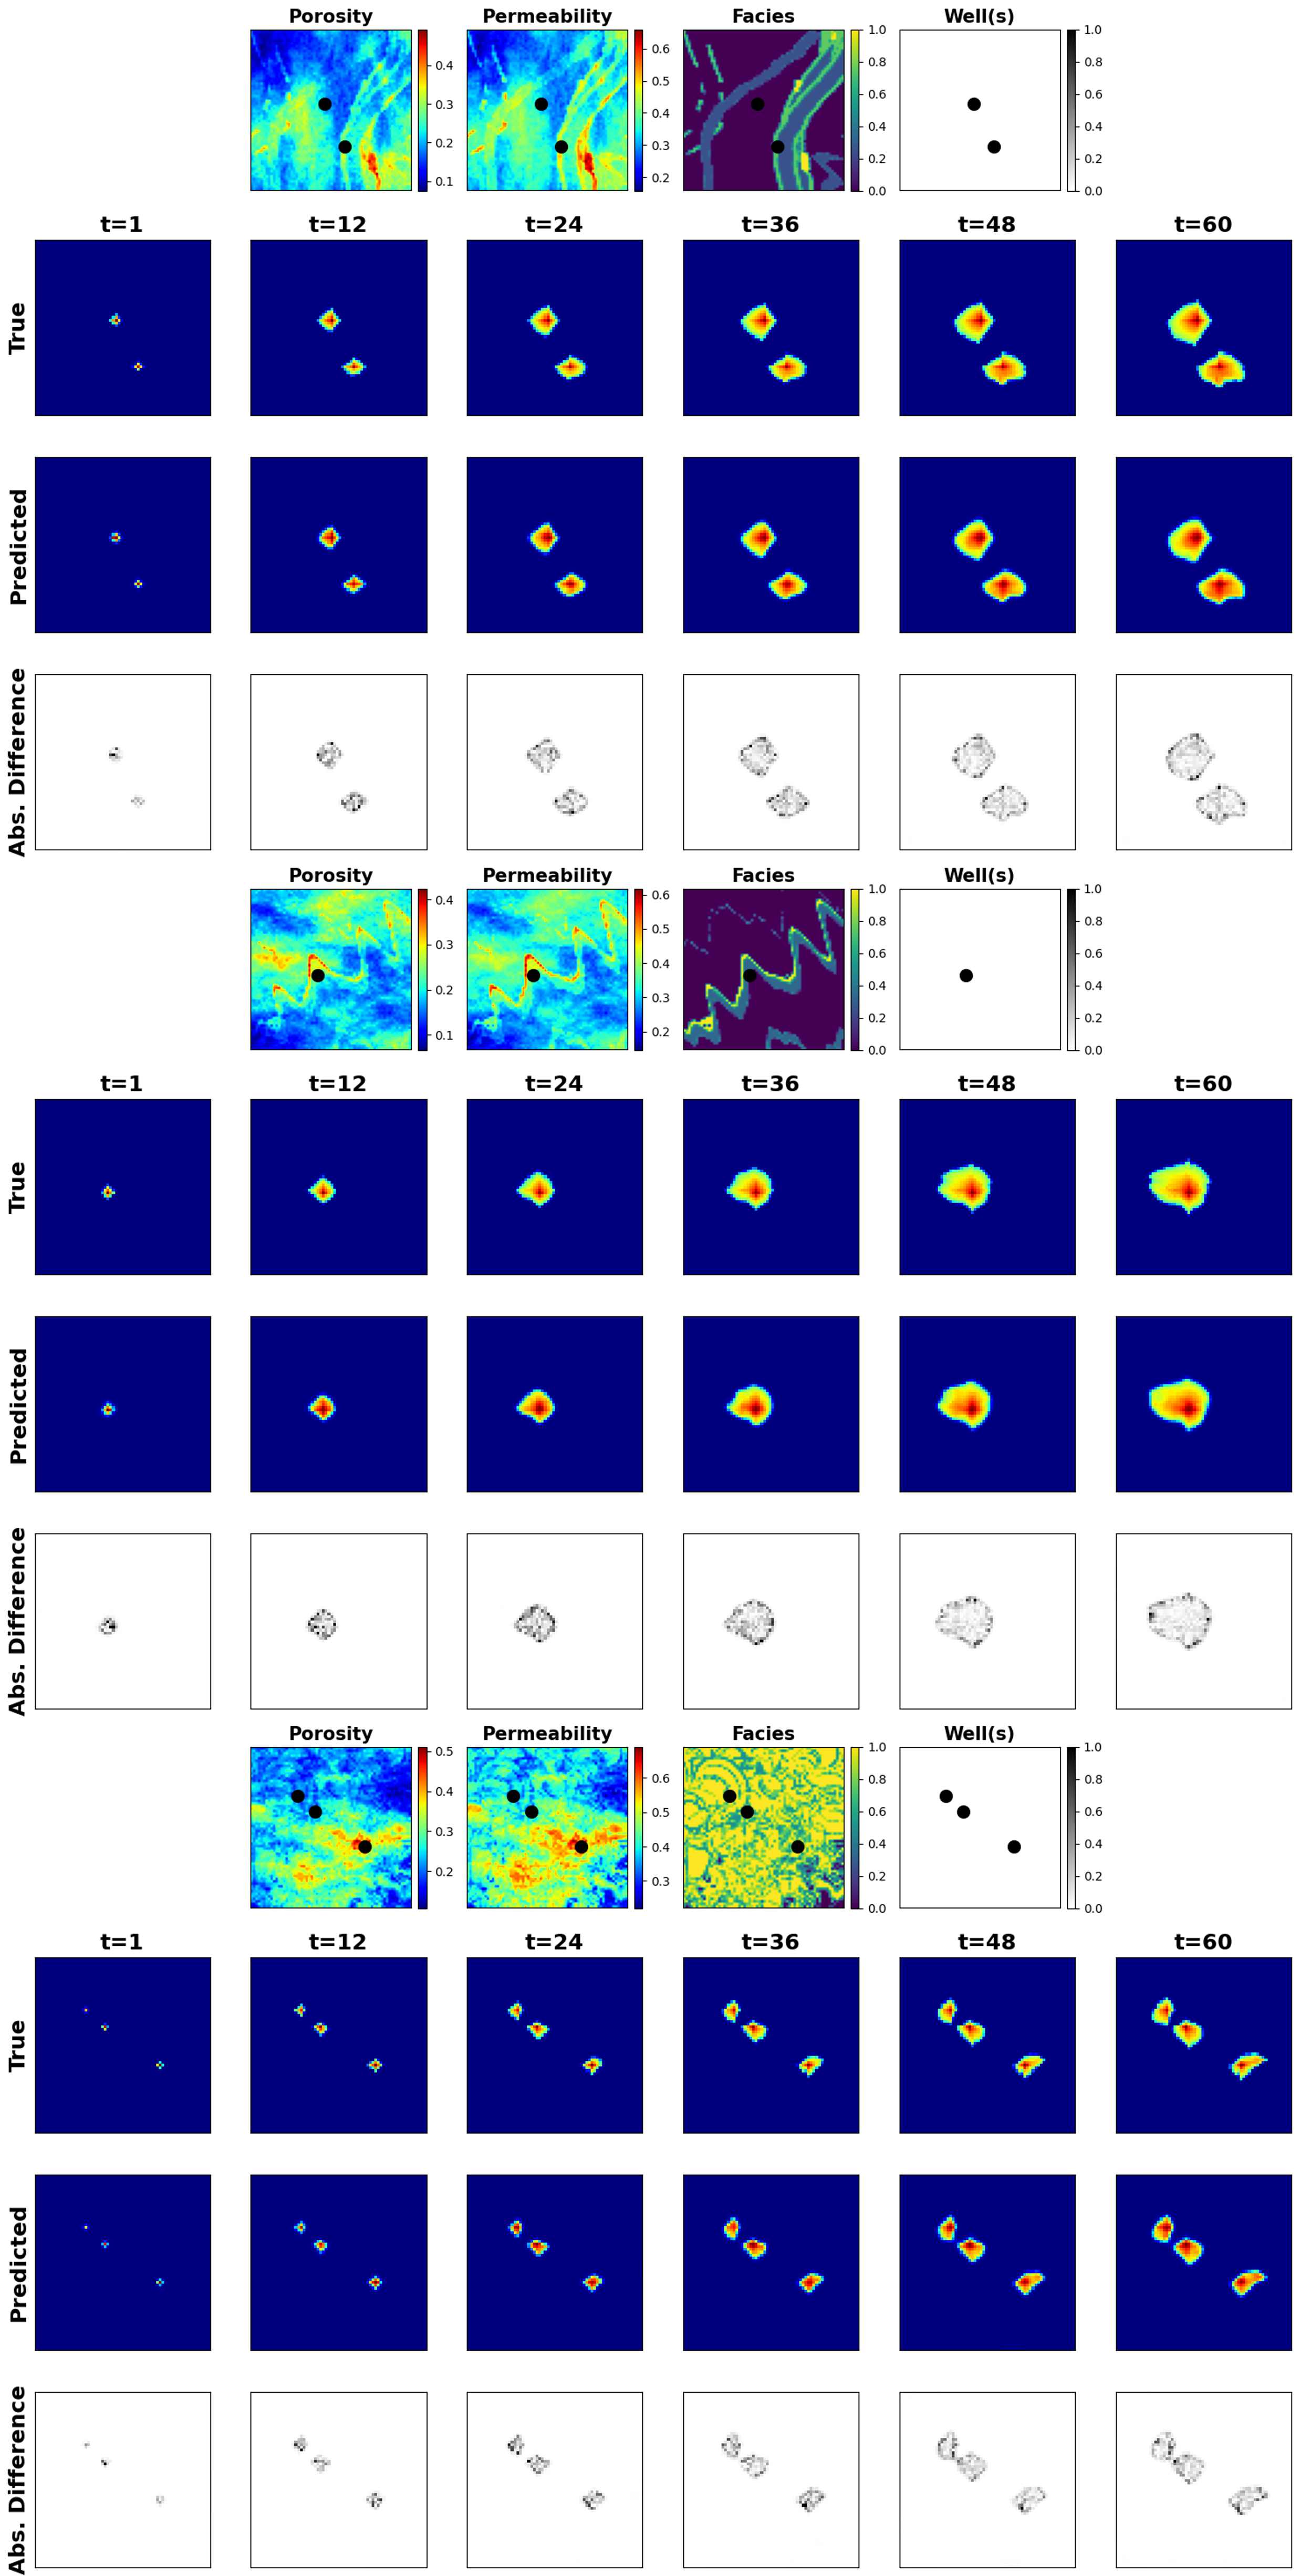
\includegraphics[width=\textwidth,height=0.95\textheight,keepaspectratio]{figures/train_sat.png}
    \caption{Saturation distribution over time for 3 random training realization. For each panel, the top row is the ground truth from the HFS, the middle row is the Stochastic pix2vid prediction, and the bottom row is the absolute difference to HFS.}
    \label{train_sat}
\end{figure}

Similarly, Figures \ref{test_pres} and \ref{test_sat} show the pressure and saturation distributions predictions along with the absolute difference to HFS for 3 testing realizations. We observe a similar performance, with an average MSE of $3.71\times10^{-4}$ and SSIM of $97.55\%$ for pressure predictions and MSE of $1.61\times10^{-3}$ and SSIM of $96.19\%$ for saturation predictions. This indicates that the Stochastic pix2vid model is generalizable and achieves on par performance with HFS at a fraction of the computational cost.

It is interesting to note that the Stochastic pix2vid model is trained on a triple-loss function with MSE, MAE and SSIM. For both training and testing cases, we see that the average MSE for pressure is higher than that of saturation, while the opposite is true for the average SSIM. This can be attributed to the fact that there are more pixel-wise variations in pressure predictions, thus the loss focuses on matching those individual pixel-wise values. On the other hand, for saturation predictions, the contrast, luminance, and structure play a bigger role in the prediction that the pixel-wise intensity values. Therefore, it is important to take into account both metrics for training and validating spatiotemporal subsurface prediction models.

\begin{figure}
    \centering
    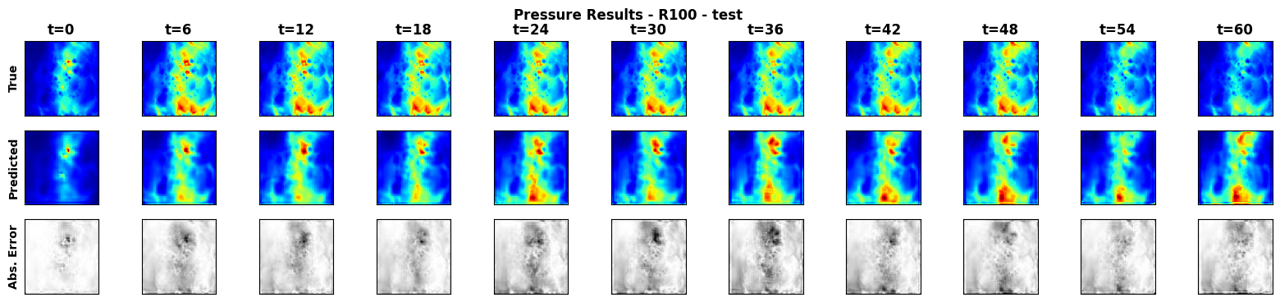
\includegraphics[width=\textwidth,height=0.95\textheight,keepaspectratio]{figures/test_pres.png}
    \caption{Normalized pressure distribution over time for 3 random testing realization. For each panel, the top row is the ground truth from the HFS, the middle row is the Stochastic pix2vid prediction, and the bottom row is the absolute difference to HFS.}
    \label{test_pres}
\end{figure}

\begin{figure}
    \centering
    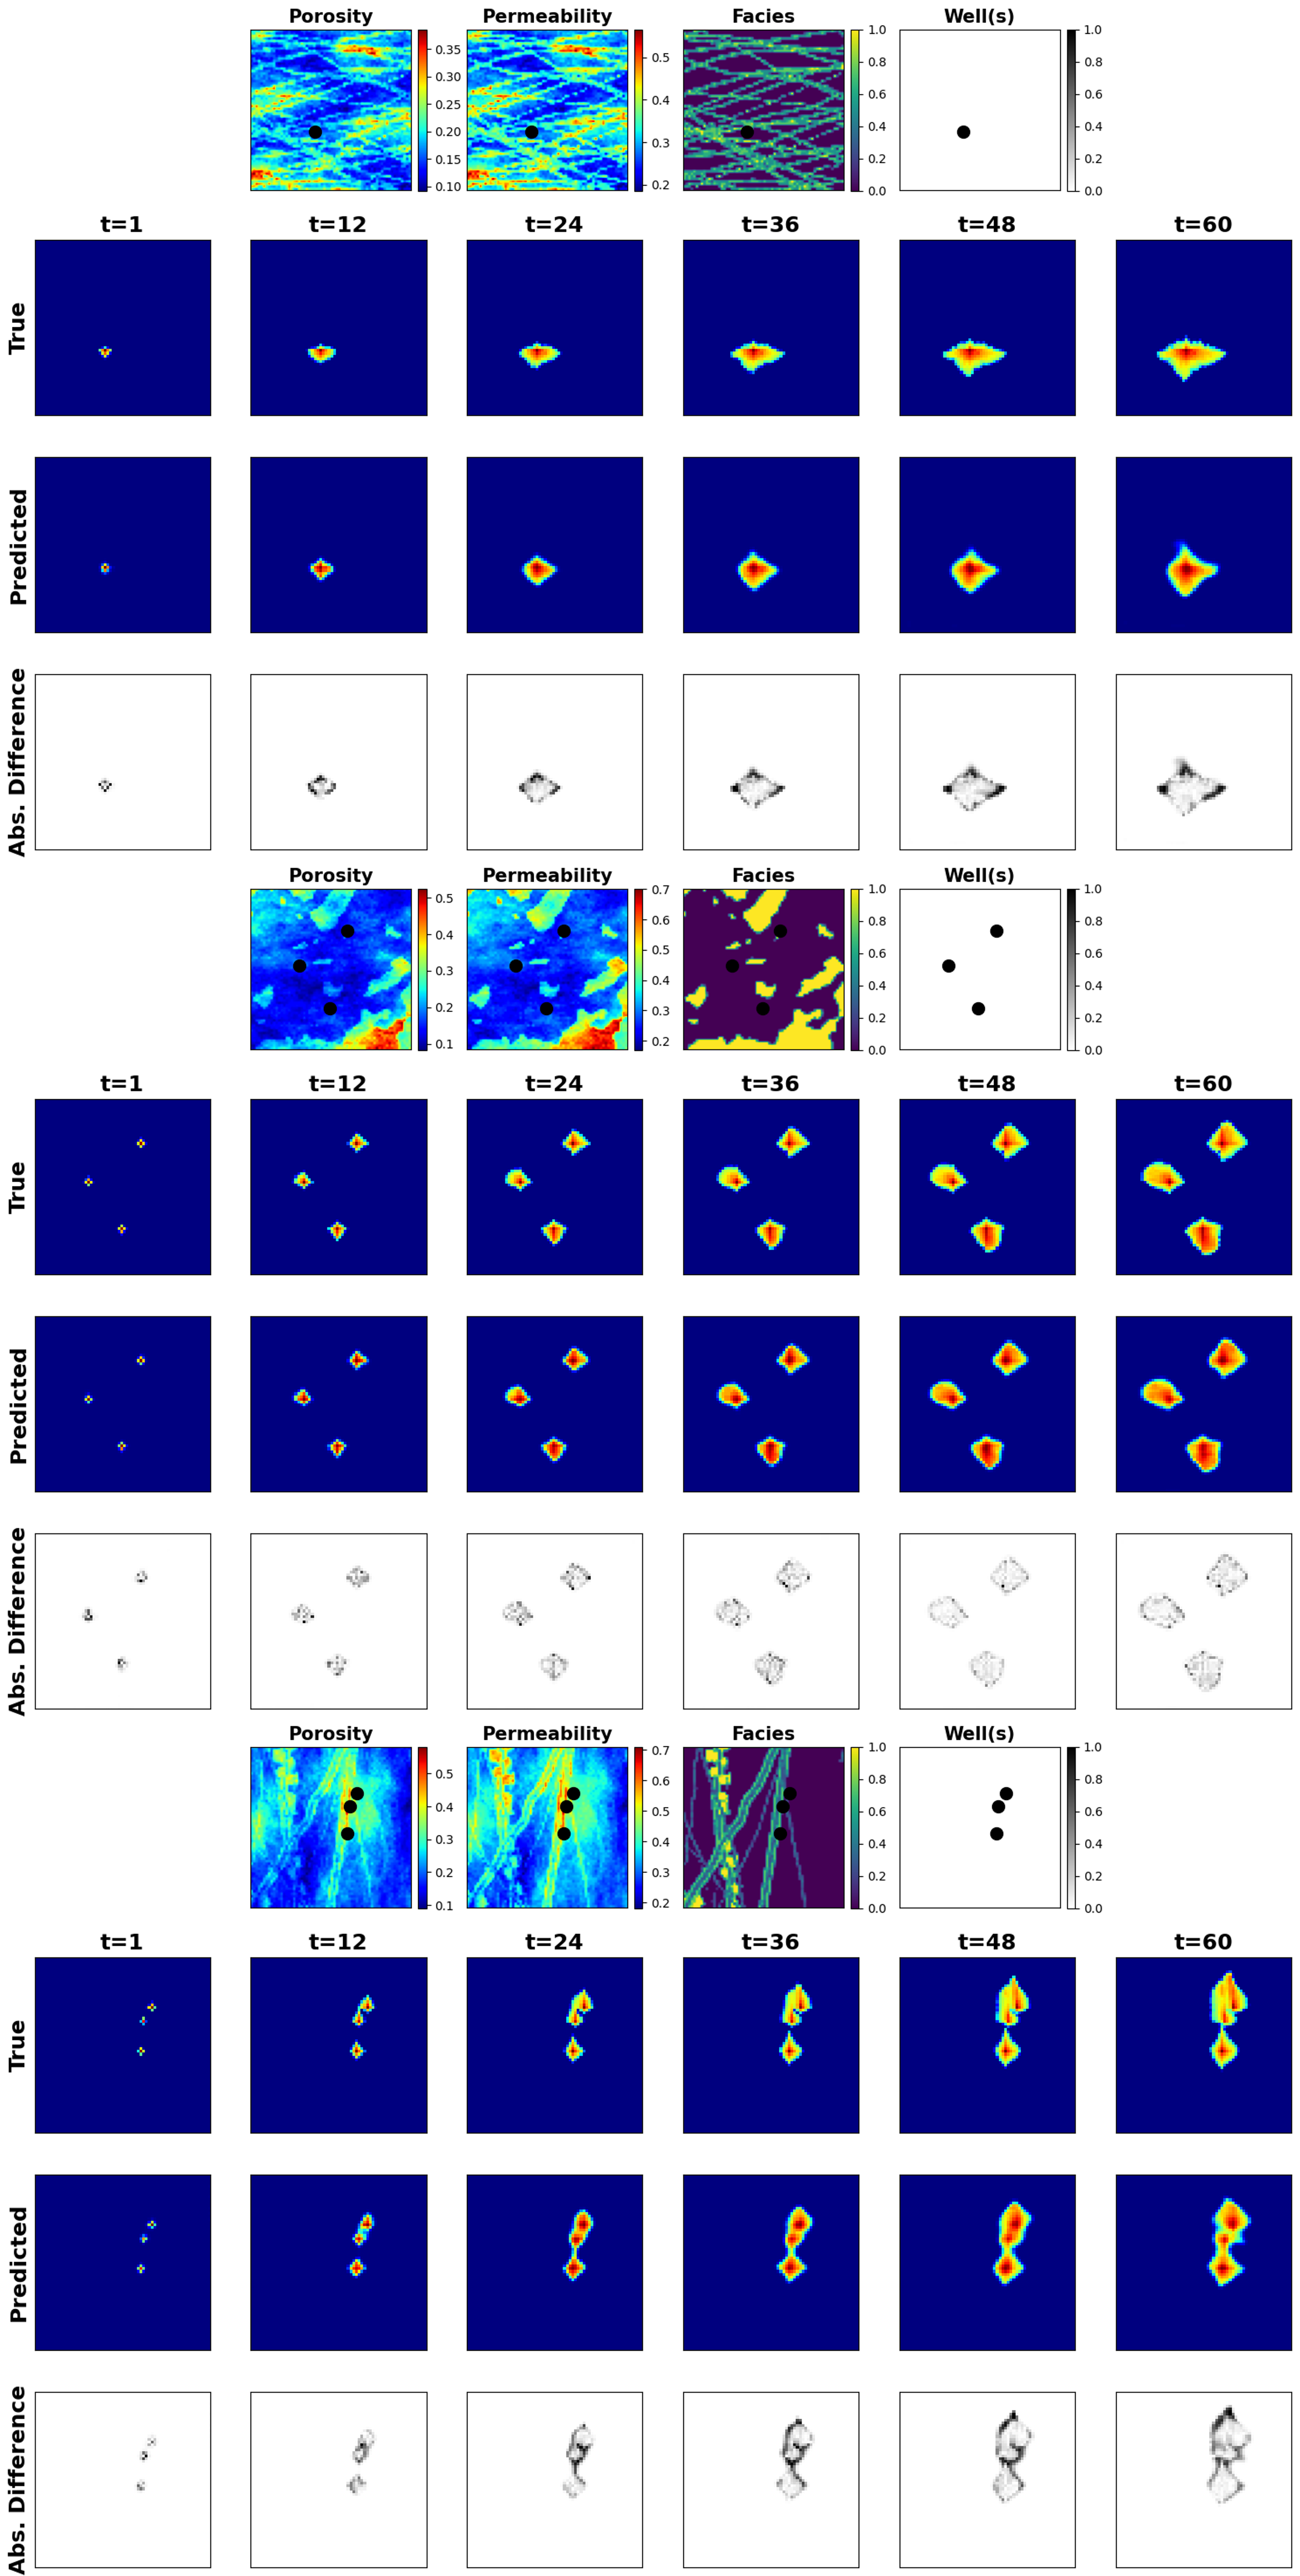
\includegraphics[width=\textwidth,height=0.95\textheight,keepaspectratio]{figures/test_sat.png}
    \caption{Saturation distribution over time for 3 random testing realization. For each panel, the top row is the ground truth from the HFS, the middle row is the Stochastic pix2vid prediction, and the bottom row is the absolute difference to HFS.}
    \label{test_sat}
\end{figure}

From Section 2.2, the first step of the Stochastic pix2vid model is to take the static geologic realizations, $m$, and compresses them into a latent space representation, $z_m$, using the spatial encoder structure. Figure \ref{feature_maps} show a random selection of latent feature maps, along with their superposition on the porosity and facies distribution. This can be interpreted as an analog to the attention head mechanisms recently developed in transformer-based architectures \cite{vaswani2017attention}. We observe that the latent feature maps are essentially learning the injection location(s) and direction of flow based on the geologic distributions. Thus, proving that the Stochastic pix2vid model is learning multiphase flow physics and dynamic reservoir behavior appropriately.

\begin{figure}
    \centering
    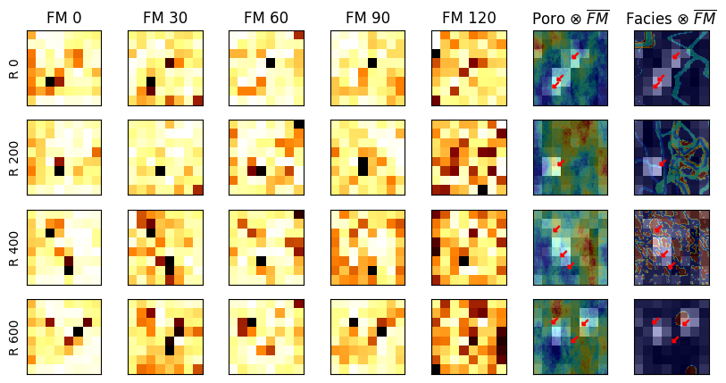
\includegraphics[width=\textwidth]{figures/feature_maps.png}
    \caption{Five random feature maps (FM) of $z_m^3$ for 4 random realizations. Their average is superimposed on top of the porosity and facies distributions to show the attention mechanism of the encoder. Bright colors represent higher attention and dark colors represent lower attention.}
    \label{feature_maps}
\end{figure}

These results imply that our Stochastic pix2vid is capable of learning the spatiotemporal relationship between the static geologic models and the dynamic reservoir response. Thus, our image-to-video architecture can outperform current image-to-image and encoder-recurrent-decoder architectures to provide improved reservoir behavior prediction closer to that of traditional numerical simulation. To quantify the uncertainty in predictions, a comparison of true ($d$) versus predicted ($\hat{d}$) response for pressure and saturation distributions for the testing data is shown in Figure \ref{r2ci}. The average $R^2$ over time is approximately $99\%$ with narrow $95\%$ prediction bands that recursively narrow over time. From Figure \ref{r2ci} we observe the advantage in implementing recursive refining of predictions over time with recurrent residual connections in the spatiotemporal decoder network, thus reducing the spatiotemporal uncertainty in the predictions.

\begin{figure}
    \centering
    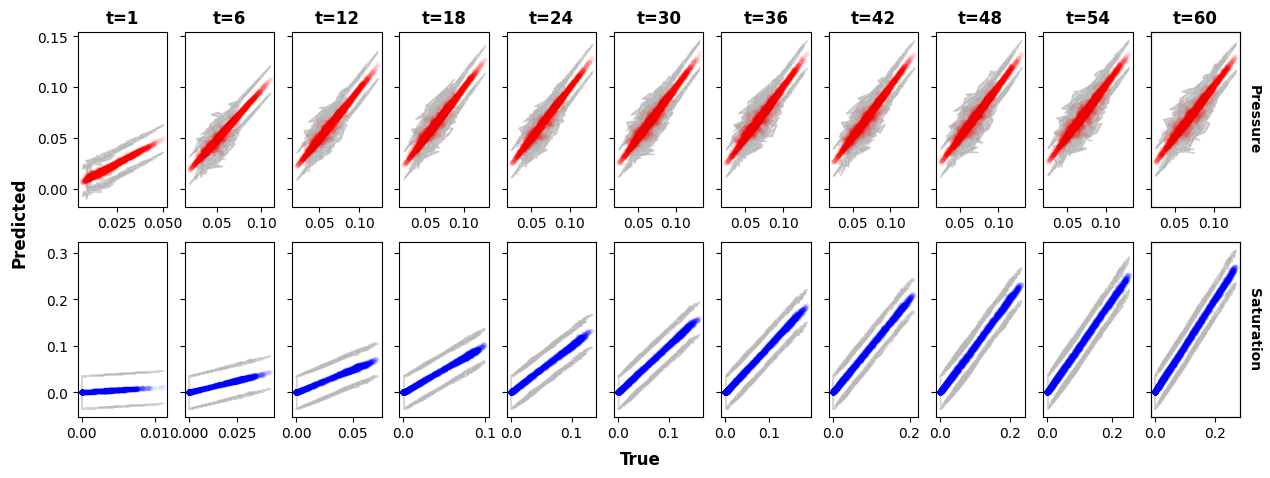
\includegraphics[width=\textwidth]{figures/r2ci.png}
    \caption{True versus predicted average normalized pressure (top) and saturation (bottom) over time for the testing data. The gray portion represents the 95\% confidence bands, which narrow over time.}
    \label{r2ci}
\end{figure}

CO$_2$ saturation and pressure buildup fronts are important quantities for geologic CO$_2$ storage projects and are often used for regulatory oversight \cite{Li2016249, Chadwick20051385}, monitoring metrics or history matching purposes \cite{Chadwick20101171, dawuda2022geologic}. The distance between the injection well(s) and the saturation fronts represents the maximum extent of the CO$_2$ plume; however, these are often very difficult to capture accurately with data-driven proxy models. Our Stochastic pix2vid method shows greater absolute error on and around the plume fronts compared to within the plumes. However, the overall shape and intensity of the pressure and saturation distributions over time is very well captured for all realizations despite being highly heterogeneous. Therefore, the Stochastic pix2vid model can be used as a reliable replacement for expensive numerical reservoir simulations, especially in cases where large number of runs are required to obtain dynamic estimates (e.g., well placement and control optimization, history matching, uncertainty quantification).

%%========= subsection 3.4 =========%%
\textbf{3.4 Discussion}

In our Stochastic pix2vid model, the encoder block is composed of separable convolutions, squeeze and excite layers, and instance normalization. These three particular implementations allow for precise parameterization of the geologic realization into a latent representation, without mixing the effects of Gaussian-distributed properties against binary of binomial-distributed properties. Using recursive residual ConvLSTM layers, the decoder block iteratively predicts each dynamic state, or video frame, from the concatenation of the previous dynamic latent representation and the intermediate encoding parameterizations. Thus, our architecture makes the proxy model an image-to-video prediction formulation for dynamic reservoir states from a static geologic realization.

To further demonstrate the effectiveness of our Stochastic pix2vid model for geologic CO$_2$ storage operations, we plot the cumulative pixel-wise CO$_2$ saturation as a surrogate for the cumulative CO$_2$ volume injected. For all training and testing realizations, Figure \ref{co2_pvi} shows the sum of pixel-wise CO$_2$ saturation and the probability density function (PDF) of the true versus predicted saturations. We observe an $R^2$ of 98\% for training and 96\% for testing in the cumulative CO$_2$ saturation of true versus predicted results, and a conformable PDFs for both training and testing.

\begin{figure}
    \centering
    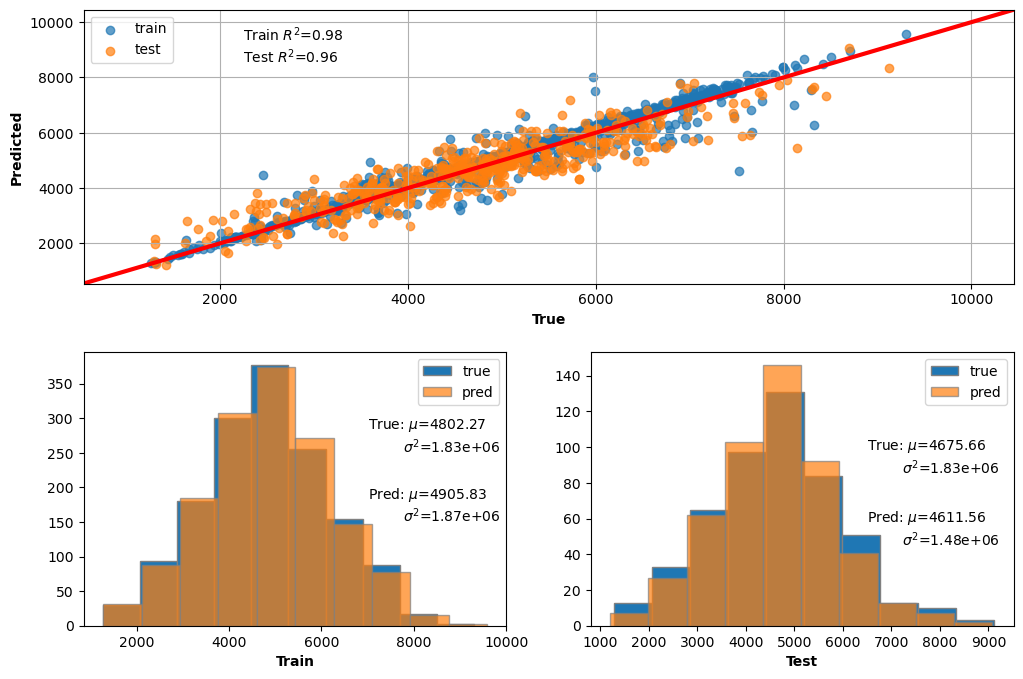
\includegraphics[width=\textwidth]{figures/co2_pvi.png}
    \caption{(Top) True vs. predicted cumulative CO$_2$ volume injected via pixel-wise saturation. (Bottom) True vs. predicted distributions of cumulative CO$_2$ saturation for training (left) and testing (right).}
    \label{co2_pvi}
\end{figure}

Our Stochastic pix2vid method has several limitations. In order to learn the spatiotemporal relationships between input images and output videos, the model requires substantial amounts of training data, which in turn require expensive physics-based numerical simulation runs. Moreover, the method would require retraining in order to apply to a different subsurface flow and transport problem, increasing the time required for generating the training data and the time required to retrain the model. One major limitation is the inability to predict for timesteps beyond those present in the training data. The architecture of the Stochastic pix2vid is designed to reconstruct only the 11 timesteps present in $d$, therefore it is capable of interpolation for steps in between the training timesteps, but incapable to forecast beyond $t=$5 years (60 months). Lastly, the method is designed for images at the resolution of $64\times64$ pixels, and preprocessing is required to reshape training data of other dimensions to this size.

%%==================================%%
%%             CONCLUSIONS          %%
%%==================================%%
\section*{\textbf{4 Conclusions}}

We develop a deep learning-based spatiotemporal proxy model to provide efficient flow predictions for a large-scale GCS operations to support optimum decision making. Our proposed method, Stochastic pix2vid, introduces the use of a spatiotemporal convolutional-recurrent architecture for dynamic predictions of CO$_2$ pressure and saturation distributions over time from a static geologic realization representing the subsurface uncertainty model. The framework is developed as an image-to-video prediction, which is an under-determined estimation problem. Specifically, the implementation expands upon the architectures of current encoder-recurrent-decoder models and provides a fast and accurate proxy as a replacement for physics-based numerical reservoir simulation.

The spatiotemporal proxy is applied to a synthetic 2D GCS project with multiple uncertain geologic scenarios and random number and location of injection well(s). A total of 1,000 geologic models are obtained from a variety of possible geologic scenarios including fluvial, turbidite, and deepwater lobe systems. The spatial distribution of porosity, permeability and facies, and the spatial location of the injector well(s) are used as the input data. The proxy model is used to predict the dynamic reservoir response over time, namely the video frames, corresponding to the dynamic CO$_2$ pressure and saturation distributions, which are obtained offline for training using HFS. The total training time is 88 minutes on a single NVIDIA Quadro M6000 GPU, and predictions are obtained with 98-99\% accuracy within approximately 4.6 milliseconds, compared to the approximate 30 seconds required for HFS, a $6,500\times$ speedup. 

There are several opportunities for future work. First, an extension to 3D geologic models and their corresponding dynamic predictions is key to scaling up this method for real-world applications. Similarly, although the Stochastic pix2vid proxy model is only trained for GCS prediction, it is applicable for a range of processes such as ground-water, compositional, geothermal, or conventional oil and gas systems. Moreover, it is possible to extend the Stochastic pix2vid model from a data-driven mapping to a PINN by including the discretized form of the governing PDE in the loss function and minimizing the residuals. Another future opportunity is to test the performance of the Stochastic pix2vid model on unseen timesteps, either interpolating the training timesteps or extrapolating beyond the training timesteps. Furthermore, the Stochastic pix2vid model can be used as a proxy in workflows for history matching and closed-loop reservoir management. 

\section*{\textbf{Reproducibility}}
The code will be made publicly available on the author's repository (github.com/misaelmmorales and github.com/GeostatsGuy).

\section*{\textbf{Funding}}
This research did not receive any specific grant from funding agencies in the public, or not-for-profit sectors.

\section*{\textbf{Declarations}}
The authors declare no conflict of interests.

\section*{\textbf{Acknowledgements}}
The authors thank the Digital Reservoir Characterization Technology (DIRECT) and Formation Evaluation (FE) Industry Affiliate Program at the University of Texas at Austin for supporting this work.

\bibliography{references.bib}

\end{document}